\chapter{A gray box analysis of the effect of torque feedback during cycling under lateral perturbations} \label{hapticFB}

\section{Introduction}
\section{Methods}

\subsection{Bicycle Model}
The bicycle model used is the so called Whipple-Carvalho model the dynamics of which have been expressed in a set of linearized equations by \citet{meijaard2007linearized}. In the original model three assumptions are made. The first is that the rider is rigidly attached in the saddle with the mass of the arms and legs acting as a point. Secondly, the contact betweeen tire and ground is modelled as a non slipping rolling point contact meaning that the wheels can rotate without lateral slip. Lastly it is assumed that the total energy of the system is preserved. The resulting non-holonomic mechanical model has three velocity degrees of freedom, the forward speed, the rear frame roll rate \ensuremath{\dot{\phi}} and the steering rate \ensuremath{\dot{\delta}}.
\begin{figure}[ht]
    \centering
    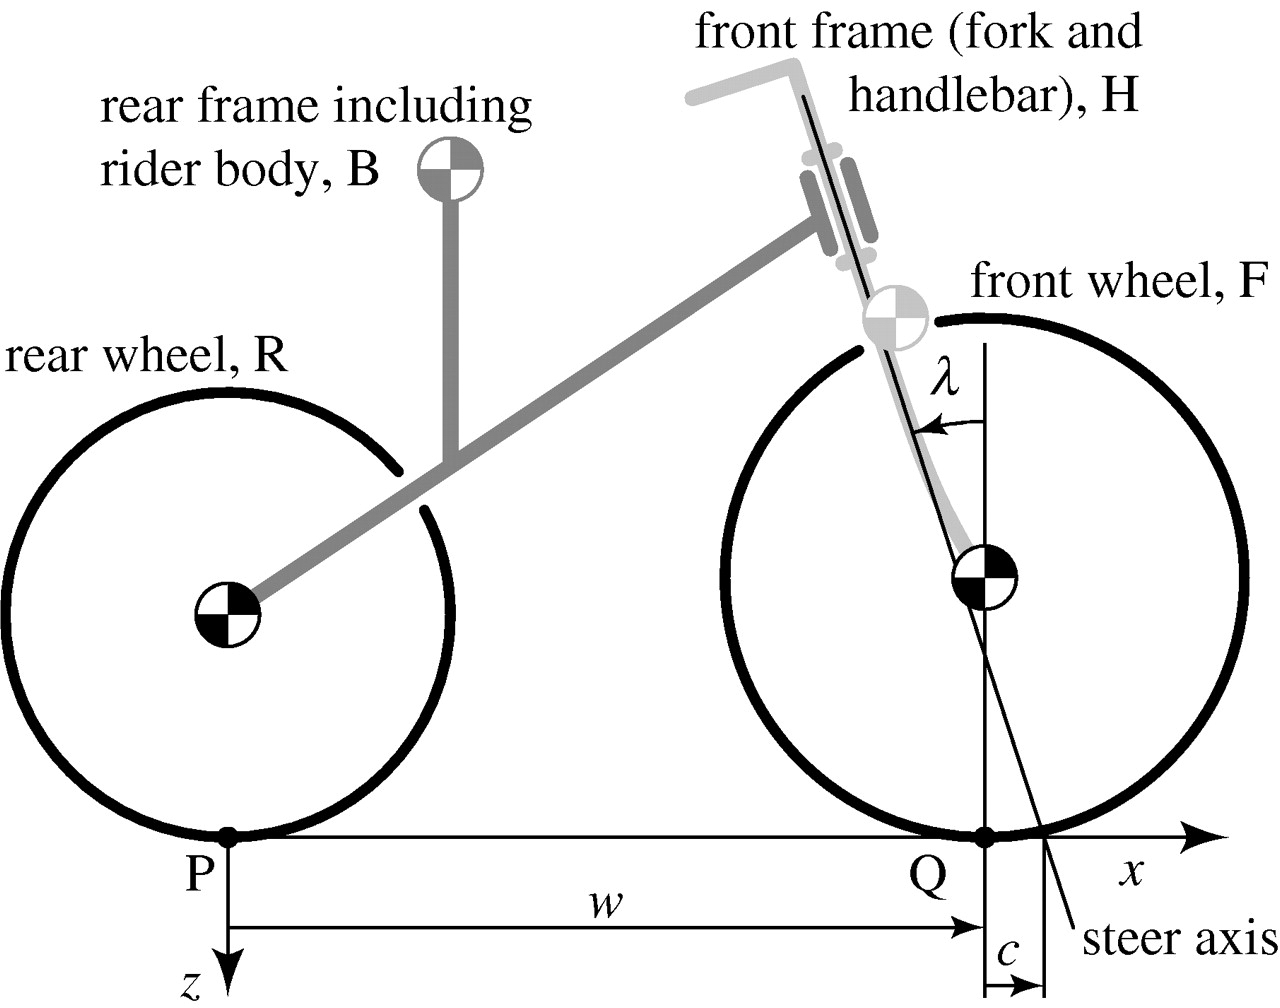
\includegraphics[scale=0.3]{images/figure3_1.png}
    \caption{ The Whipple-Carvalho bicycle model consists of four rigid bodies: rear wheel R, rear frame B, front frame H and front wheel F connected via hinges. The center of mass locations are expressed relative to the x - and z -coordinates shown (with origin at P and y pointing towards the reader). The other parameters shown are the steer axis tilt \ensuremath{\lambda}, wheelbase \ensuremath{w} and trail \ensuremath{c}. The model at its most expanded form is described by 25 parameters.\cite{meijaard2007linearized}}
    \label{fig:figure2}
\end{figure}
The lateral motion is described by  two coupled second order differential equations given by \cref{eq:paper1}.
\begin{equation}
    \mathbf{M} \ddot{q}+v \mathbf{C}_{1} \dot{q}+\left[g \mathbf{K}_{0}+v^{2} \mathbf{K}_{2}\right] \mathbf{q}=\mathbf{f}
    \label{eq:paper1}
\end{equation}

where \ensuremath{\mathbf{q}} is a vector containing the roll and steer angles, \ensuremath{\mathbf{f}} is a vector containing the roll and steer torques, \ensuremath{g} is the gravitational acceleration and \ensuremath{\mathbf{M},\;v\mathbf{C}_{1},\;g \mathbf{K}_{0}+v^{2} \mathbf{K}_{2}} are the "mass", "damping" and "stiffness" ratios in matrix form respectively. The entries in the constant coefficient matrices  \ensuremath{\mathbf{M},\mathbf{C}_{1}, \mathbf{K}_{0},  \mathbf{K}_{2}} are calculated from a set of 25 bicycle parametrers related to inertial and design properties of the steer by wire bicycle (see \cref{tb:paper1}).

To determine the stability of the open loop system in a straight ahead motion the characteristic polynomial derived from
\begin{equation}
    \operatorname{det}\left(\mathbf{M} \lambda^{2}+v \mathbf{C}_{1} \lambda+g \mathbf{K}_{0}+v^{2} \mathbf{K}_{2}\right)=0
    \label{eq:paper2}
\end{equation}

is solved for a forward speed range from 0 to 10 \si{\meter\per\second} where \ensuremath{\lambda} are the eigenvalues of the system (see \cref{fig:paper2}). The two intresting eigenmodes defined by the locus plot are the weave and capsize. The weave corresponds to an oscillatory mode as can be seen by the existance of imaginary parts and represents a motion in which the bicycle sways about its heading. The oscillatory motions exponentially fades when forward speed is larger than 4.39 \si{\meter\per\second}. The capsize on the other hand has an eigenvector dominated by lean and leads to a gradual roll drift to infinity when the eigenvalue crosses the zero line around 6.67 \si{\meter\per\second}.
\begin{figure}[ht]
    \centering
    \captionsetup{justification=centering,margin=2cm}

    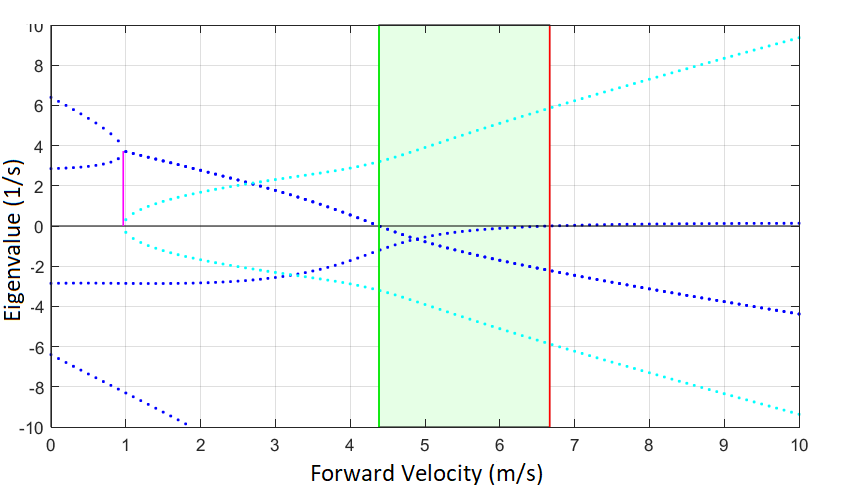
\includegraphics[scale=0.6]{images/root_locus_steerbywire.png}
    \caption{Root locus plot of the steer by wire bicycle. Dotted blue lines indicate the real part of the eigenvalues while dotted cyan show the imaginary part. The stable region corresponds to speeds  \ensuremath{4.39\lessapprox v \lessapprox 6.67\; \si{\meter\per\second}}}
    \label{fig:paper2}
\end{figure}
Since in the experimental setup the task could not be isolated to purely balance the equations are extended to include heading. Heading is defined as a linear combination of steer angle and steer rate as expressed by \citet{meijaard2007linearized} in \cref{eq:paper3}. Additionally, the bike is assumed to be controlled only by a steering torque because according to both \citet{moore2012human} and \citet{weir1973manual}  the rear frame roll angle is mainly
controlled by steering. 

\begin{equation}
    \dot{\psi}=\frac{v \delta+c \dot{\delta}}{w} \cos \lambda
    \label{eq:paper3}
    \end{equation}

When modelling the feedback off case of the steer-by-wire bicycle the dynamics of the plant need to change accordingly. In that configuration the forcing steering input is directly proportional to steering acceleration times the inertia of upper handlebar assembly, for this reason the second of the set of equations in \ref{eq:paper1} is replaced by :
\begin{equation}
    I_{F_{xx}}\ddot{\delta} = T_{\delta}
\end{equation}

 For control purposes \cref{eq:paper1} is expressed in state space form with state vector \ensuremath{\mathbf{x}=[\dot{\phi}, \dot{\delta}, \phi, \delta, \psi]^{T}}, forcing input \ensuremath{\mathbf{f}=T_{\delta}} and ouput equal to the full state.
 \begin{equation}
    \dot{\mathbf{x}}=\mathbf{A} \mathbf{x}+\mathbf{B} T_\delta + \mathbf{H} w
    \label{eq:bikeEOM}
\end{equation}
\begin{equation}
    \mathbf{y}=\mathbf{C} \mathbf{x}+\mathbf{D} \mathbf{f}
\end{equation}
where matrices \ensuremath{A,B,C,D} are defined by:
\begin{align}
    \mathbf{A} &=\begin{bmatrix}
        -\mathbf{M}^{-1}v\mathbf{C}_{1} & -\mathbf{M}^{-1}(g \mathbf{K}_{0}+v^{2}\mathbf{K}_{2}) \\
        {\mathbf{I}_2}                    & {\mathbf{0}} \\  {\begin{matrix} {0} & { \frac{c cos\lambda}{w}}\end{matrix}} &  {\begin{matrix} 0 & { \frac{v cos\lambda}{w}}\end{matrix} } 
    \end{bmatrix} , \mathbf{B}=\left[ \begin{array}{c}{\mathbf{M}^{-1}} \\ {\mathbf{0}}\end{array}\right] \\
    \mathrm{C} &= {\mathbf{I}_5} , \mathrm{D}=\mathbf{0} 
\end{align}

where \ensuremath{\mathbf{H}} is the matrix defining the dynamics of the lateral disturbance w. 

\subsection{Rider Control Model}\label{subsec:rider_model}

In order to investigate the effects of the torque feedback loop attributed to the golgi tendon organs a rider control model is created. The complete high level overview of the model is shown in \cref{fig:paper3}.
\begin{figure}[ht]
    \centering
    \captionsetup{justification=centering,margin=2cm}

    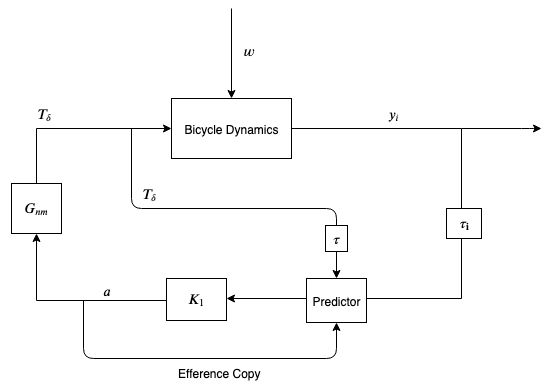
\includegraphics[scale=0.6]{images/rider_block_overview.jpg}
    \caption{Block diagram of the complete rider-bicycle model. \ensuremath{G_{nm}} is the neuromuscular dynamics block. \ensuremath{K_1} is a pure Gain block working on the extended output plus the torque feedback   while \ensuremath{\tau_i} are the delays of each output \ensuremath{y_i} attributed to different sensory organs of the human body. } 
    \label{fig:paper3}
\end{figure}

\ensuremath{G_{nm}} is the neuromuscular transfer function and works as a second order filter to simulate the limitations of the human response. In state space form this block is expressed by :

\begin{align}
\dot{x}_{nm} &= \begin{bmatrix}0 & 1 \\ -\omega^2 & -2\zeta\omega\end{bmatrix} \begin{bmatrix} T_\delta \\ \dot{T}_\delta\end{bmatrix} + \begin{bmatrix} 0 \\ \omega^2\end{bmatrix} a \\
    y_{nm} &= \begin{bmatrix}1 & 0\end{bmatrix} \begin{bmatrix} T_\delta \\ \dot{T}_\delta\end{bmatrix}
        \label{eq:gnmBLOCK}
\end{align}

where \ensuremath{\zeta} is the damping coefficient and \ensuremath{\omega_c} is the cutoff frequency. These  parameters were chosen according to activations dynamics present in the shoulder joint \cite{happee2008posture}.

The steer angle and steer rate feedback is attrubuted to the muscle spindles, while the torque feedback is made possible with the help of the golgi tendon organs. The roll and heading angle come from the visual system. Lastly the roll rate feedback is attributed to the vestibular system. 

The bicycle model of \cref{eq:bikeEOM} is combined with the neuromuscular dynamics block of \cref{eq:gnmBLOCK} to create a combined  plant with state \ensuremath{x=[\dot{\phi}, \dot{\delta}, \phi, \delta, \psi, T_\delta \dot{T}_\delta]^{T}} ,input \ensuremath{a} and \ensuremath{w} and output \ensuremath{y=[\dot{\phi}, \dot{\delta}, \phi, \delta, \psi, T_\delta]^{T}}. In order to make possible the implementation of the predictor which is discrete in nature the state space representation of the combined plant is discretized with a time step of 0.001 \si{\second}. The equivalent model block diagram is shown in \cref{fig:paper4}.

\subsubsection{The reafferent optimal predictor}
Many strategies to counter time delays have been proposed in literature. The most basic predictor is the Smith Predictor, which has been explored in motor control research by \citet{miall1993cerebellum}. The smith predictor compensates for time delays through the use of an internal forward model of the controlled dynamics and an internal model of the sensory delay pathways. The forward model works by utilizing an efferent signal of the control input while the comparison between prediction and measurement is trying to simulate the human's ability to distingush between reafference and exafference.  Unfortunetly the  most basic smith predictor scheme does not work for unstable open loop systems \cite{guzman2006interactive}. In this work a modification to the normal smith predictor scheme is suggested. In place of the forwrard model an optimal tapped delay line is used that forward simulates the amount of steps according to the model of sensory delay. This works like a resetting forward model that is updated every time step by the delayed state so the predictor loop does not become unstable. A tapped delay line without the smith  correction can still work and has been implemented by \citet{van2001adaptive} for modelling stance control but it leads to predictions that do not contain any amount of the effect of the disturbance on the state. The predictor structure used in this work  can be seen in \cref{fig:paper4}.



 \begin{figure}[ht]
    \centering
    \captionsetup{justification=centering,margin=2cm}

    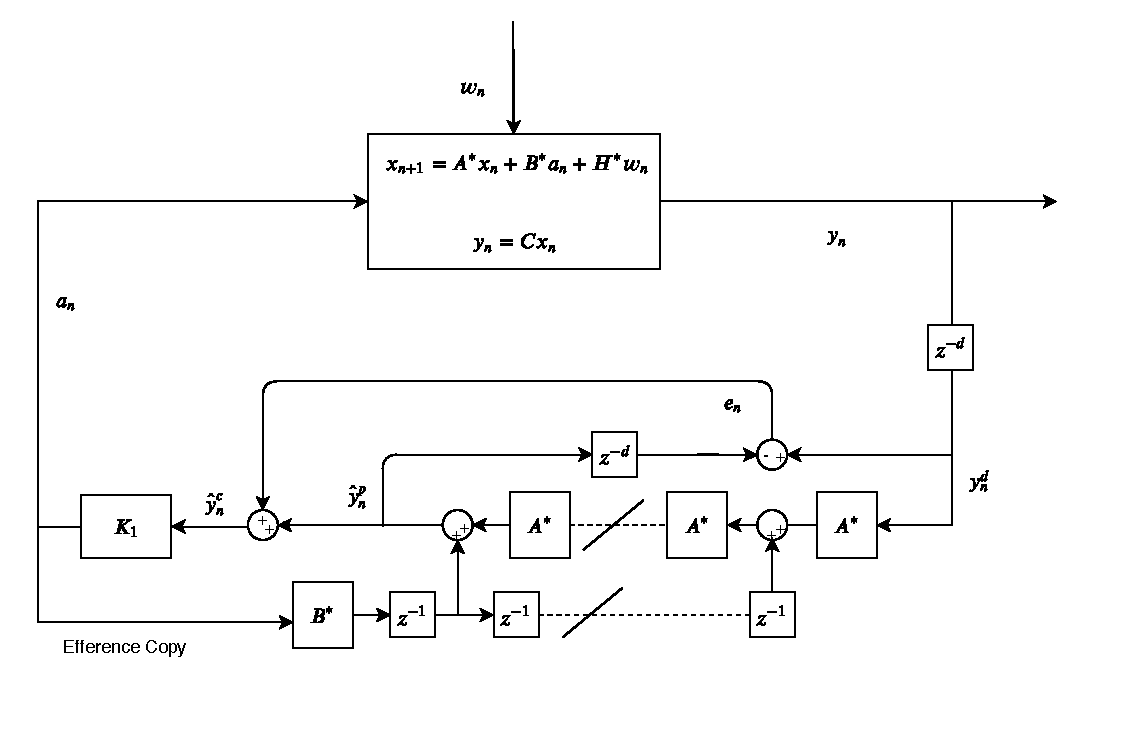
\includegraphics[scale=0.6]{images/discrete_block.pdf}
    \caption{Equivalent block diagram of the bicycle-rider system in discrete time. \ensuremath{A^*} ,\ensuremath{B^*} are the discretized matrices of the combined plant dynamics while d is the amount of time delay in number of time steps. The delayed output measurement is forwared in time in the tapped delay line to produce the first undelayed estimate of the output \ensuremath{\hat{y}^p} , which is again delayed through a model of the time internal time delay. The difference between this re-delayed prediction with the delayed measurements creates the error \ensuremath{e} which is added back to  \ensuremath{\hat{y}^p}  to create the final corrected prediction \ensuremath{\hat{y}^c} }
    \label{fig:paper4}
\end{figure}

\subsection{Parameter Estimation }

In order to assess the effectiveness of the torque feedback loop, three models of incremental complexity are used. In the first the feedback pathways are fed into the controller without delays. In the second delays are added. The third one compensates for time delays by the use of the predictor discribed above. The three models have the  controller gains as free parameters. The gains are estimated by fitting the model output into the non-parametric dataset derived in \cite{dialynaseffect}.  The gains were estimated by minimization of the cost function 
\begin{equation}
    V_{N}(\boldsymbol{\theta})=\frac{1}{N} \sum_{k=1}^{N}\left[5\cdot\left(\hat{y}^{\delta}_k(\mathbf{\theta})-y^\delta_k\right)^{2}+\left(\hat{y}^{\psi}_k(\mathbf{\theta})-y^\psi_k\right)^{2}+8\cdot10^{-4}\left(\hat{y}^{T_\delta}_k(\mathbf{\theta})\right)^2\right]
    \label{eq:cost}
    \end{equation}

where \ensuremath{\mathbf{\theta}} is a vector containing all the free parameters, \ensuremath{\hat{y}^{\delta}} and \ensuremath{\hat{y}^{\psi}} are the ouputs of the simulation for the measured external disturbance \ensuremath{w} and the vecor of parameters  \ensuremath{\mathbf{\theta}} for steer angle and heading angle respectively, while \ensuremath{y^\delta} and \ensuremath{y^\psi} are the outputs of the convolution of the measured disturbance \ensuremath{w} and the impulse response functions \ensuremath{h^\delta} and \ensuremath{h^\psi} respectively. 

The first two terms  of the cost fucntion are trying to match the steering and heading  response of the parametric model with that one of the non-parametric model, while the third on minimizes the amount of input torque generated in order to produce the best possible fit. The weights were chosen heuristically. For optimization the genetic algorithm with a fitness limit of 0.03 is first  used in order to produce a good starting parameter vector for gradient descend algotirth to take over, which finally finds the closest possible estimate of the global minimum. For the genetic algorithm a crossover fraction of 0.85  anlong with a population size 10 times the length of the parameter vector is used. Additionally, The gains attributed to the muscle spindle sensors (\ensuremath{K_\delta} and \ensuremath{K_{\dot{\delta}}}) are constrained to be only positive. The assumption is that they work like a delayed steering stiffness and damping.

The impulse response function of the median rider is used. This is determined by taking the mean impulse response function of each measured output and finding the participant which had the highest variance accounted for between the individual response and the mean accross all speed levels.
Each system was identified for three different model conditions. In the first all six feedback pathways are used including torque feedback, on the second torque feedback is exluded from the model by assuming that its corresponding gain is zero. Finally in the third, six gains are again used but the plant dynamics are modified so as to simulate the feedback off case of the experimental condition as described in \cref{subsec:rider_model}.  As metric of model validity the variance accounted for between parametric and non-parametric ouput is used, defined as
\begin{equation}
\mathrm{VAF_d}(\boldsymbol{\theta})=1 -\sum_{k=1}^{n}\left(y^{d}(k)-\hat{y}^{d}(k, \boldsymbol{\theta})^{2}\right) / \sum_{k=1}^{n}\left(y^{d}(k)^{2}\right)
\end{equation} 
where \ensuremath{d=\{\phi,\delta,\psi\}}. 

In order to asssess the importance of the torque feedback, the uncertainty of each parameter is found. Parameters with the lowest uncertainty contribute more to the fit so they are deemed more important. To find the uncertainty the covariance matrix is estimated from :
\begin{align}
    \operatorname{cov}_{\hat{\theta}}  &=V_N(\boldsymbol{\hat{\theta}})\boldsymbol{H}(\boldsymbol{\hat{\theta}})^{-1}\\ \text{with} \;\;\;\;  \boldsymbol{H}(\boldsymbol{\hat{\theta}})&= \frac{\partial^{2} V_N}{\partial \theta_{i} \partial \theta_{j}}
\end{align}

where \ensuremath{\boldsymbol{\hat{\theta}}} is the parameter vector that produces the closest estimate to the global minimum and \ensuremath{\boldsymbol{H}} is the hessian matrix numerically estimated by the gradient descend algorithm.  However, since bigger parameters are going to have naturally larger variances the diagonal values are normalized by the parameter value to produce the index of dispersion

\begin{equation}
    D_{\hat{\theta_i}}=\frac{\sigma^{2}_{\hat{\theta_i}}}{|\hat{\theta}_i|}
    \end{equation}

    where \ensuremath{\sigma^{2}_{\hat{\theta_i}}} are the diagonal elements of \ensuremath{ \operatorname{cov}_{\hat{\theta}}}.
% As far as the delays are concerned for \ensuremath{\delta} and \ensuremath{\dot{\delta}} which are attributed to the muscle spindle sensors and for the torque feedback which is attributed to the golgi tendon organs  a delay of 25 \si{\milli\second} is chosen \cite{van2002identification,de2002adaptation}. For the feedback states attributed to visual feedback such as the roll angle \ensuremath{\phi} and yaw angle \ensuremath{\psi} a much greater delay of 200 \si{\milli\second} is chosen. Finally for  the vestibular roll rate feedback a delay of 50 \si{\milli\second} is implemented \cite{barnett2013vestibular}. 
% \cite{whipple1899stability}


\section{Results}


\subsection{Zero Delay Model}
The results of the zero delay model are presented in \cref{tb:no_delay}. A fit of over 90 \% is easily achieved for both steer angle and heading, while for roll the discrepancy is larger. A  look into how the model approximates the measured rider input and bicycle states for the forward speed \ensuremath{3.6 \si{\meter\per\second}} is seen in \cref{fig:paper5}. The discrepancy in the roll angle fit can be explained by the fact that the model does not account for upper body motions which are expected to have a considerable impact on bicycle dynamics. 

\begin{figure}[!h]
    \centering
    \captionsetup{justification=centering,margin=2cm}

    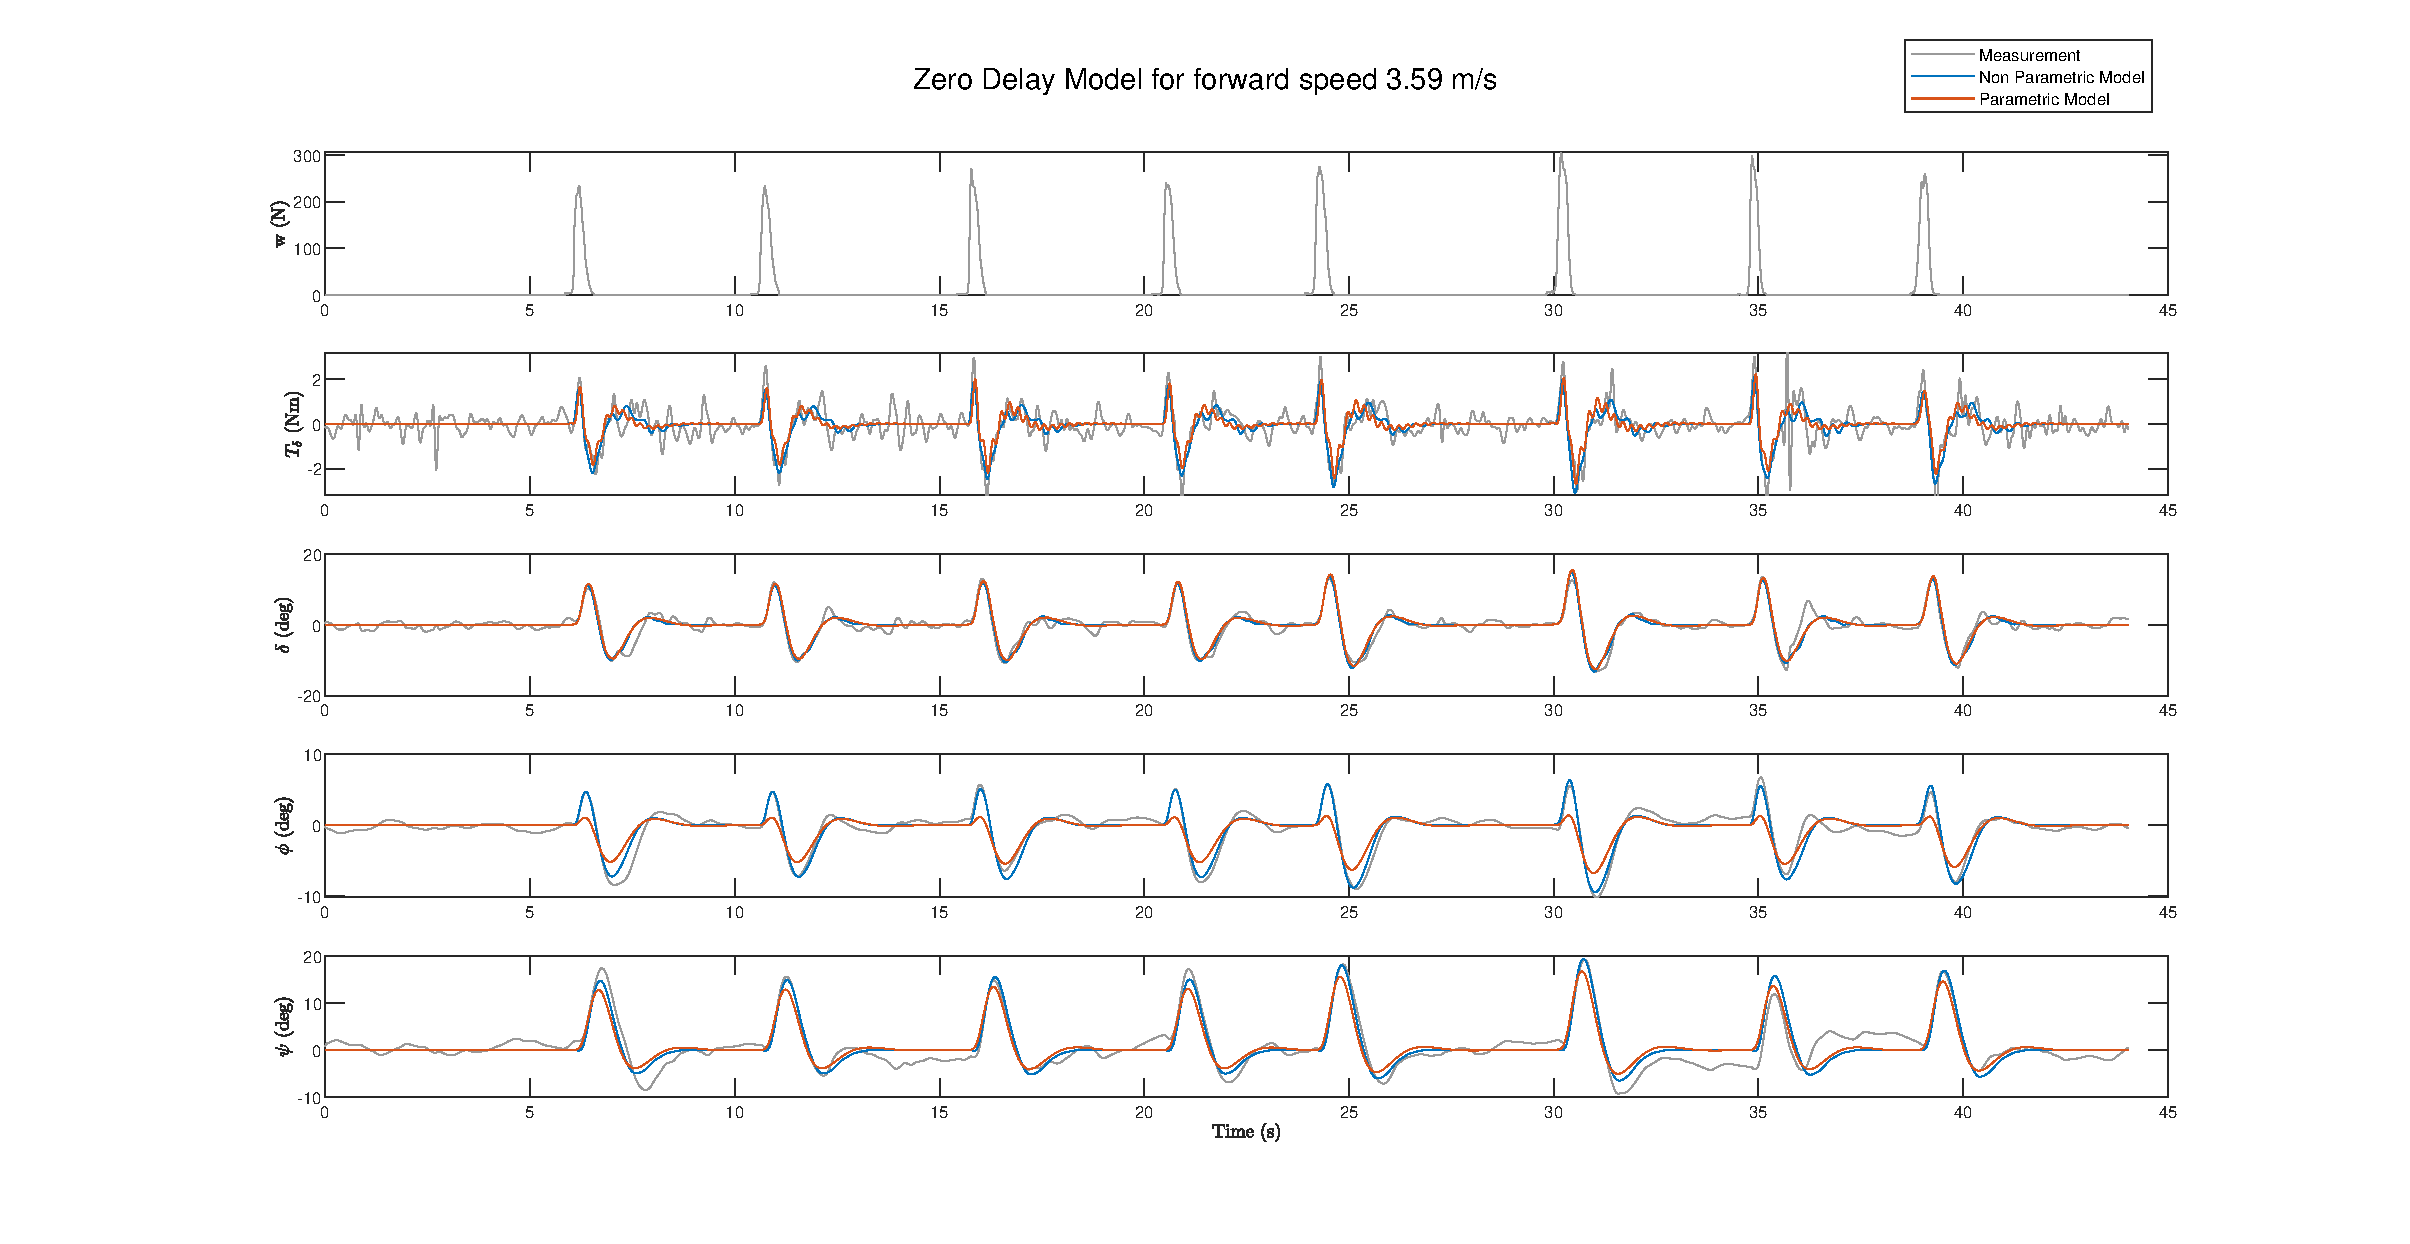
\includegraphics[width=\textwidth]{images/no_delay_result1.eps}
    \caption{Comparison between parametric model output, non-parametric model ouput and measured signals for the speed level of 3.6 \si{\meter\per\second} for the case where torque feedback activated.}
    \label{fig:paper5}
\end{figure}


From the index of dispersion it is seen that the torque feedback gain \ensuremath{K_{T_\delta}} along with the steer rate gain \ensuremath{K_{\dot{\delta}}} contribute most in the fit, since the consistently have the lowest uncertainty level among all parameters. Additionally, \ensuremath{\mathit{VAF}_\delta} drops more than 15-20\% when the feedback is turned off (see \cref{tb:no_delay}). The steering angle reponse   becomes significantly more oscillatory when the feedback is turned off (see \cref{fig:paper6}). Roll stabilization perfomance does not seem to be affected, however steering effort considerably does. Worth noting that in the experimental feeedback off case the level of fit degradation is almost non existant.

\begin{figure}[!h]
    \centering
    \captionsetup{justification=centering,margin=2cm}

    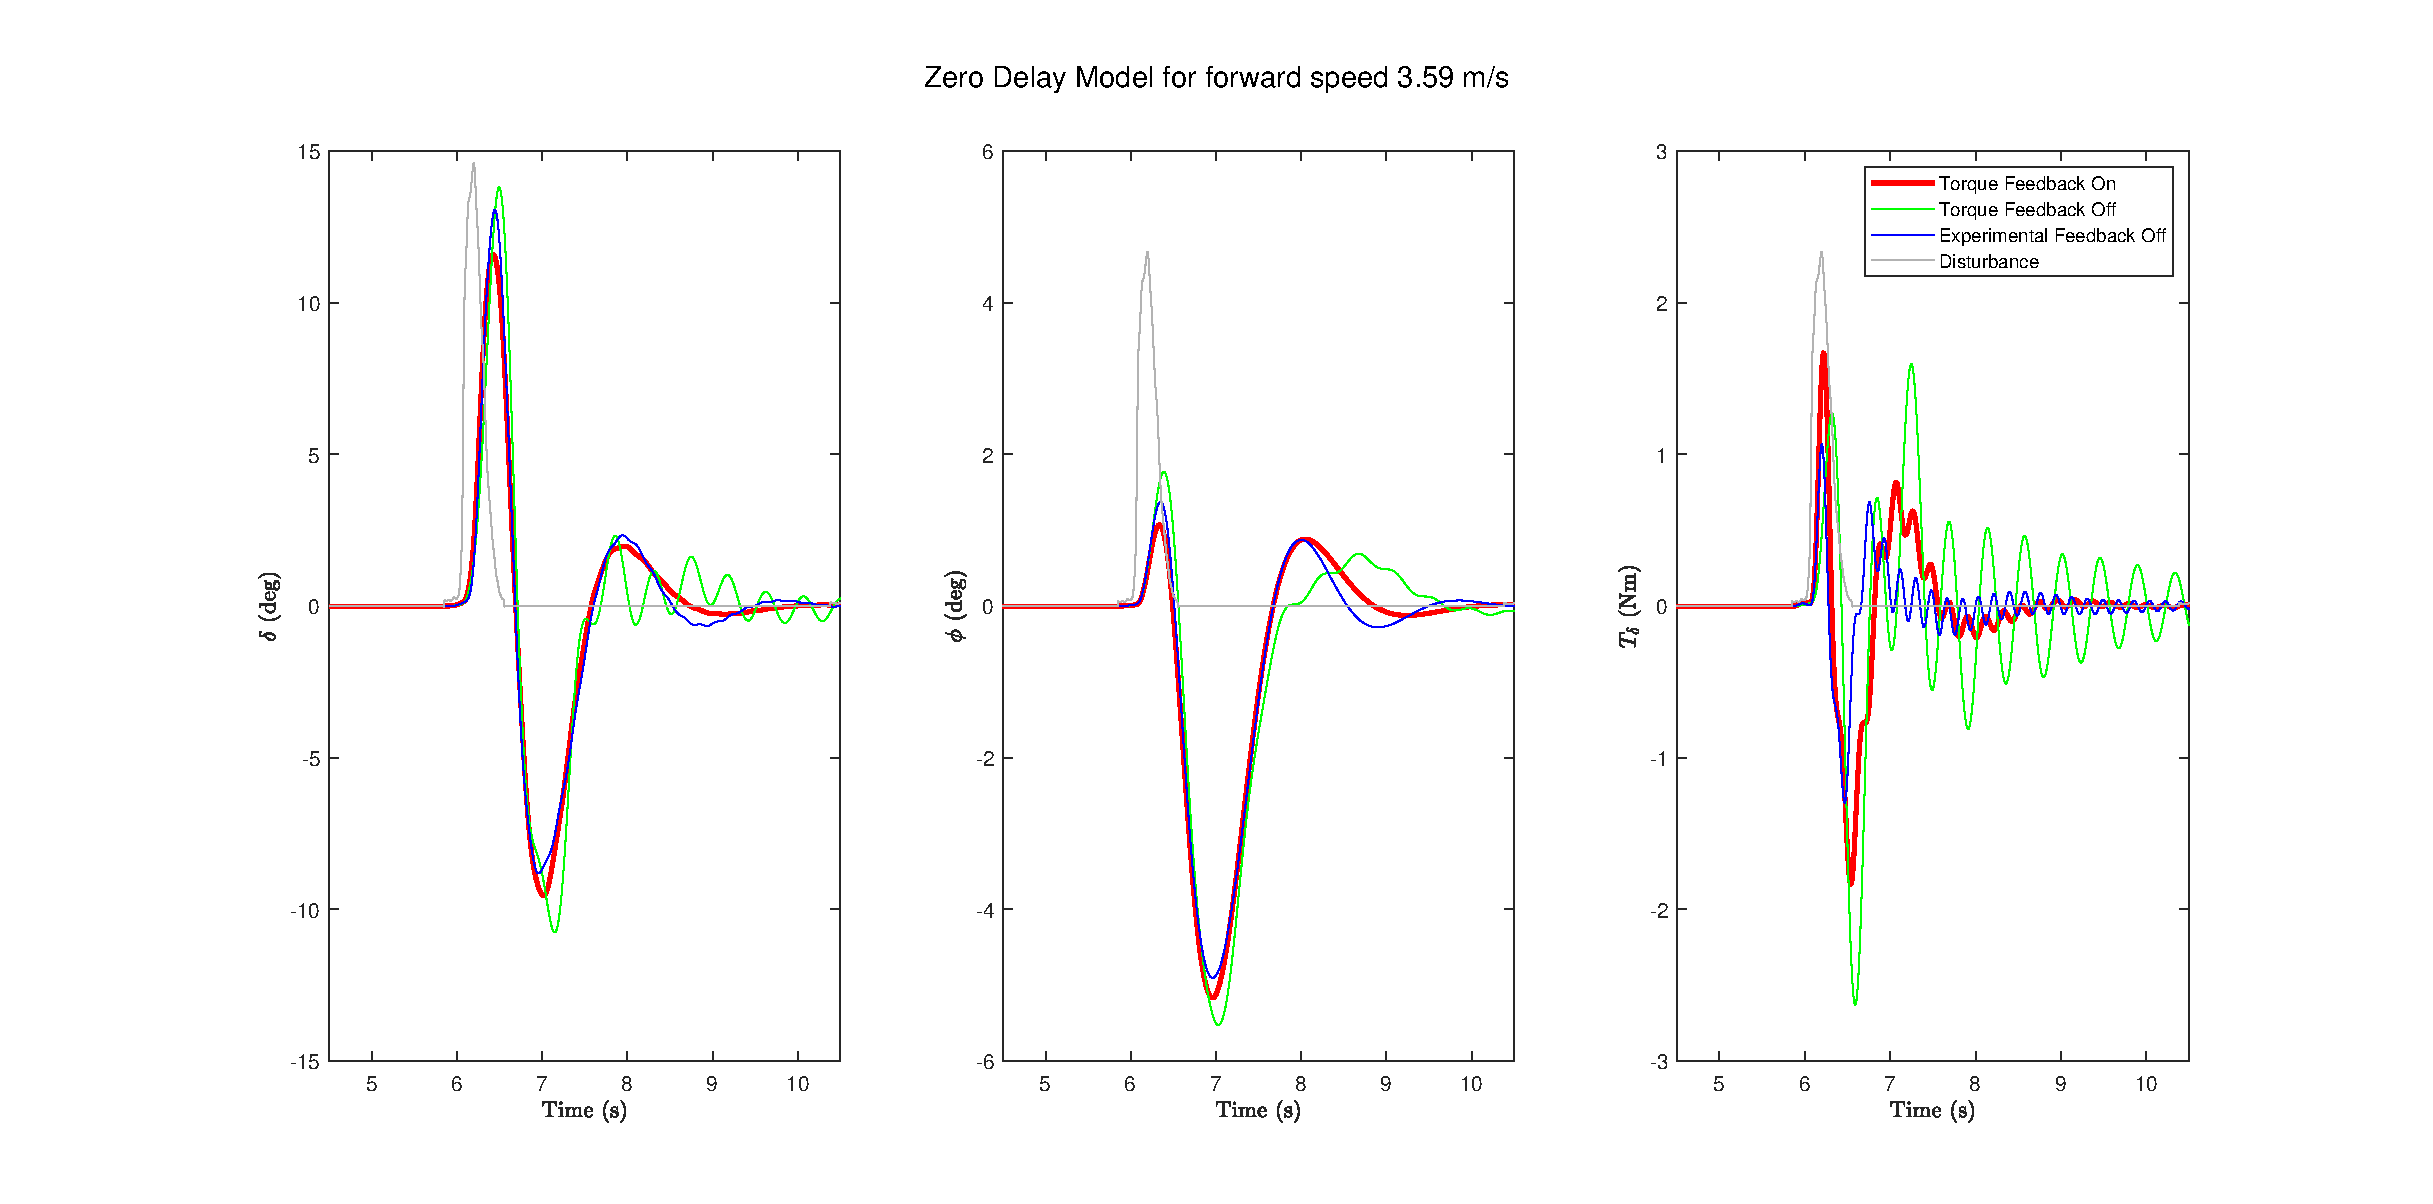
\includegraphics[width=\textwidth]{images/no_delay_fb_compare.eps}
    \caption{Steering, roll angles and input rider torque compared among torque feedback levels  for the forward speed of 3.6 \si{\meter\per\second}. The disturbance signal is not shown  to scale.}
    \label{fig:paper6}
\end{figure}



\subsection{Variable Delay Model}
The same procedure was repeated for the model but now introducing  delays in all feedback pathways. For \ensuremath{\delta} and \ensuremath{\dot{\delta}} which are attributed to the muscle spindle sensors and for the torque feedback which is attributed to the golgi tendon organs  a delay of 25 \si{\milli\second} is chosen \cite{van2002identification,de2002adaptation}. For the feedback states attributed to visual feedback such as the roll angle \ensuremath{\phi} and yaw angle \ensuremath{\psi} a much greater delay of 200 \si{\milli\second} is chosen. Finally for  the vestibular roll rate feedback a delay of 50 \si{\milli\second} is implemented \cite{barnett2013vestibular}. 

The results of the variable delay model are presented in \cref{tb:variable}.  Despite the fact that significant delay is introduced into the system the torque feedback loop manages to compensate maintining a \ensuremath{\mathit{VAF}_\delta} of over 90 \% for low speed levels (see \cref{tb:variable} and \cref{fig:paper7}). In \cref{fig:paper8} the delayed response of the rider is visible between the dotted red and bold red line. This is further exagerated in the two remaining conditions resulting in much more oscillatory steering responses with a visible impact on roll stabilization. The index of dispersion follows similar pattern as in the zero delay model, with the proportional heading and roll gains having the largest uncertainty while the steer rate and  torque feedback gain having the lowest. Between feedback on and feedback off, a much larger drop in VAF is noted. Additionally, a equally significant drop in the fit is noted for the exprimental feedback off case, which was not present in the zero delay model. 






\begin{figure}[!h]
    \centering
    \captionsetup{justification=centering,margin=2cm}

    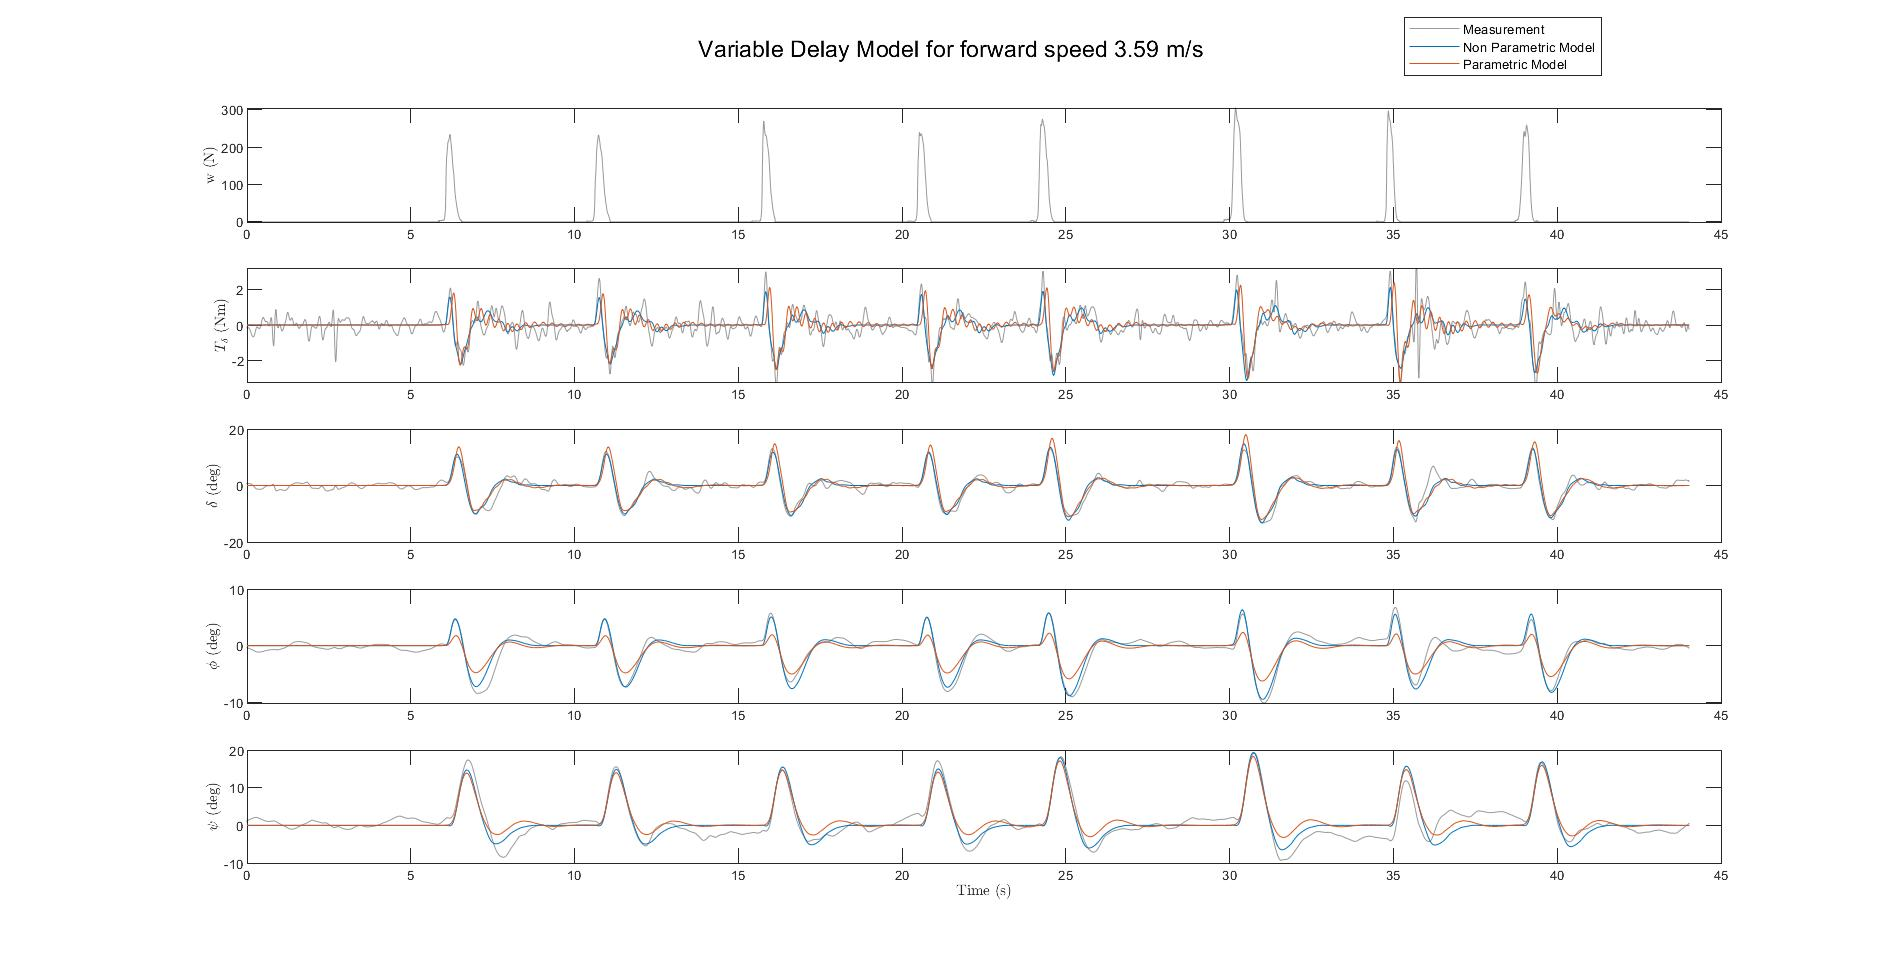
\includegraphics[width=\textwidth]{images/variable_delay_result1.eps}
    \caption{Comparison between variable delay model output, non-parametric model ouput and measured signals for the speed level of 2.8 \si{\meter\per\second} for the case where torque feedback is activated.}
    \label{fig:paper7}
\end{figure}

\begin{figure}[!h]
    \centering
    \captionsetup{justification=centering,margin=2cm}

    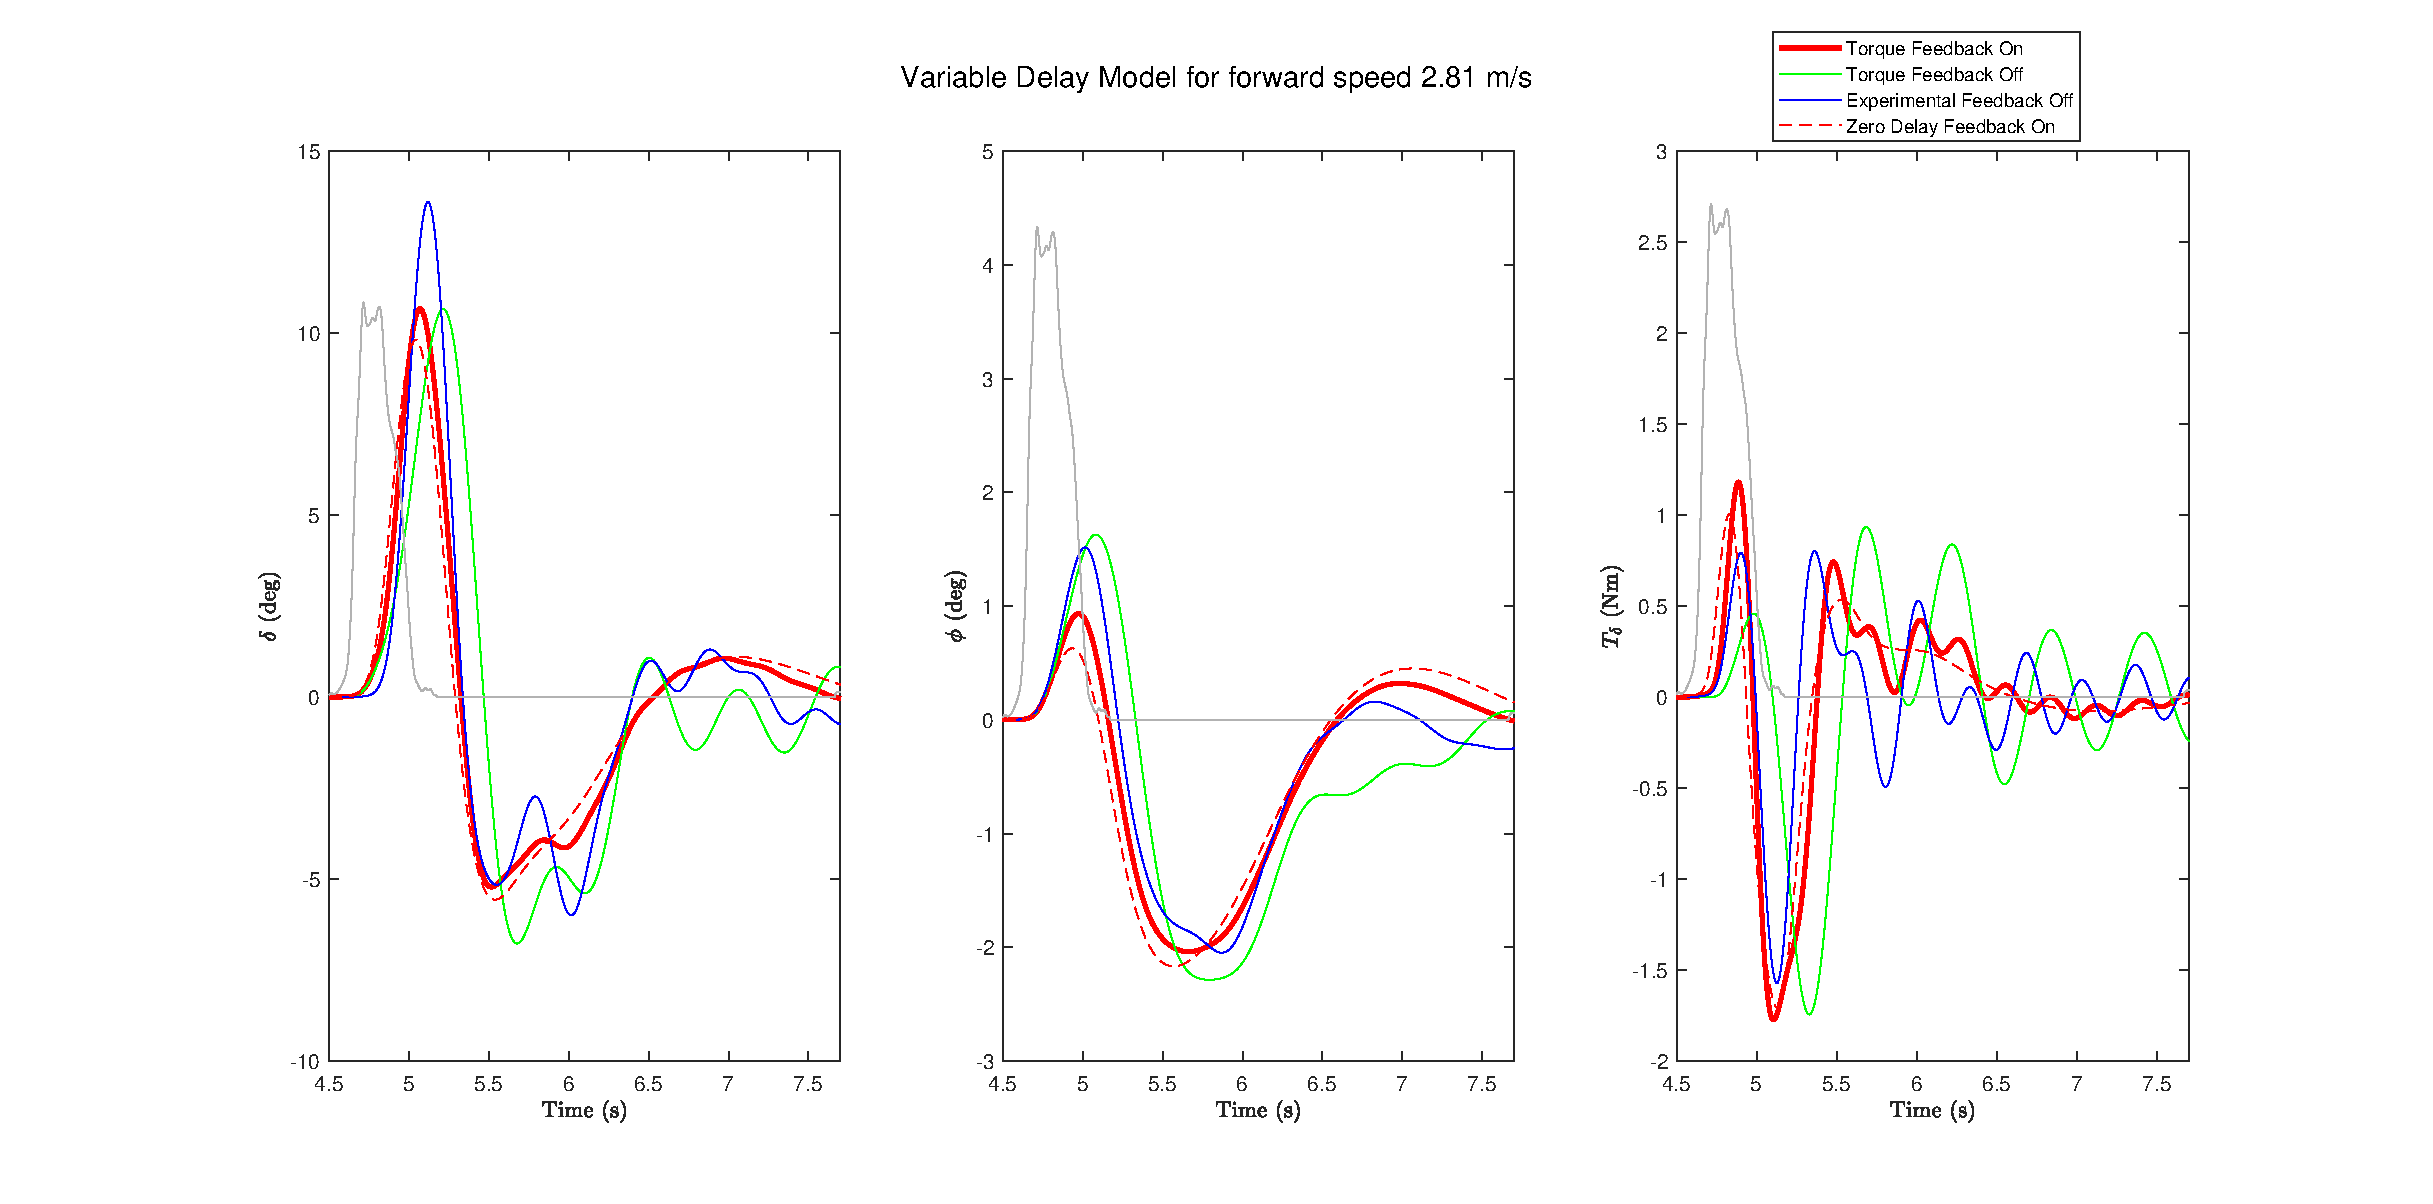
\includegraphics[width=\textwidth]{images/variable_delay_compare.eps}
    \caption{Steering, roll angles and input rider torque of the variable delay model  compared among torque feedback levels  for the forward speed of 2.8 \si{\meter\per\second}. The disturbance signal is not shown  to scale.}
    \label{fig:paper8}
\end{figure}


    \subsection{Final Model}

The final model of  \cref{fig:paper4} is implemented with a consistent time delay among sensory pathways eqaul to 50 \si{\milli\second}. Adaptation of the predictor to work with variable time delays is not part of the scope of this work. It is assumed that the inernal model of bicycle and neuromusclular dynamics along with the internal model of the inherent time delay responsible for prediction is perfect for controlling the normal bicycle dynamics. However in the experimental off case the inernal model is not updated in simulation, which that  it remains the same as a normal bike. This falls inline with what was noted during the experiements where the subjects adapted to the new bicycle dynamics instantaneously, so a full "recalibration" of the forward model is too far fetched. This way the extent to which the smith prediction principle can counter prediction model inaccuracies is also tested. 


The optimization results for the final model are presented in \cref{tb:predict_model}. From the \ensuremath{\mathit{VAF}s} and the signals shown in \cref{fig:paper9} it is visible that the quality of the fit is comparable with the ideal zero delay case. The index of dispersion follows similar trends. The drop between feedback conditions is also similar to the zero delay case. Furthermore, the steering response exhibits  the same oscillatory behaviour when torque feedback is completeley disabled. However, the predictor manages to compensate in the feedback off experimental case and achieve good fit which was not present in the model with uncompensated time delays. 

\begin{figure}[!h]
    \centering
    \captionsetup{justification=centering,margin=2cm}

    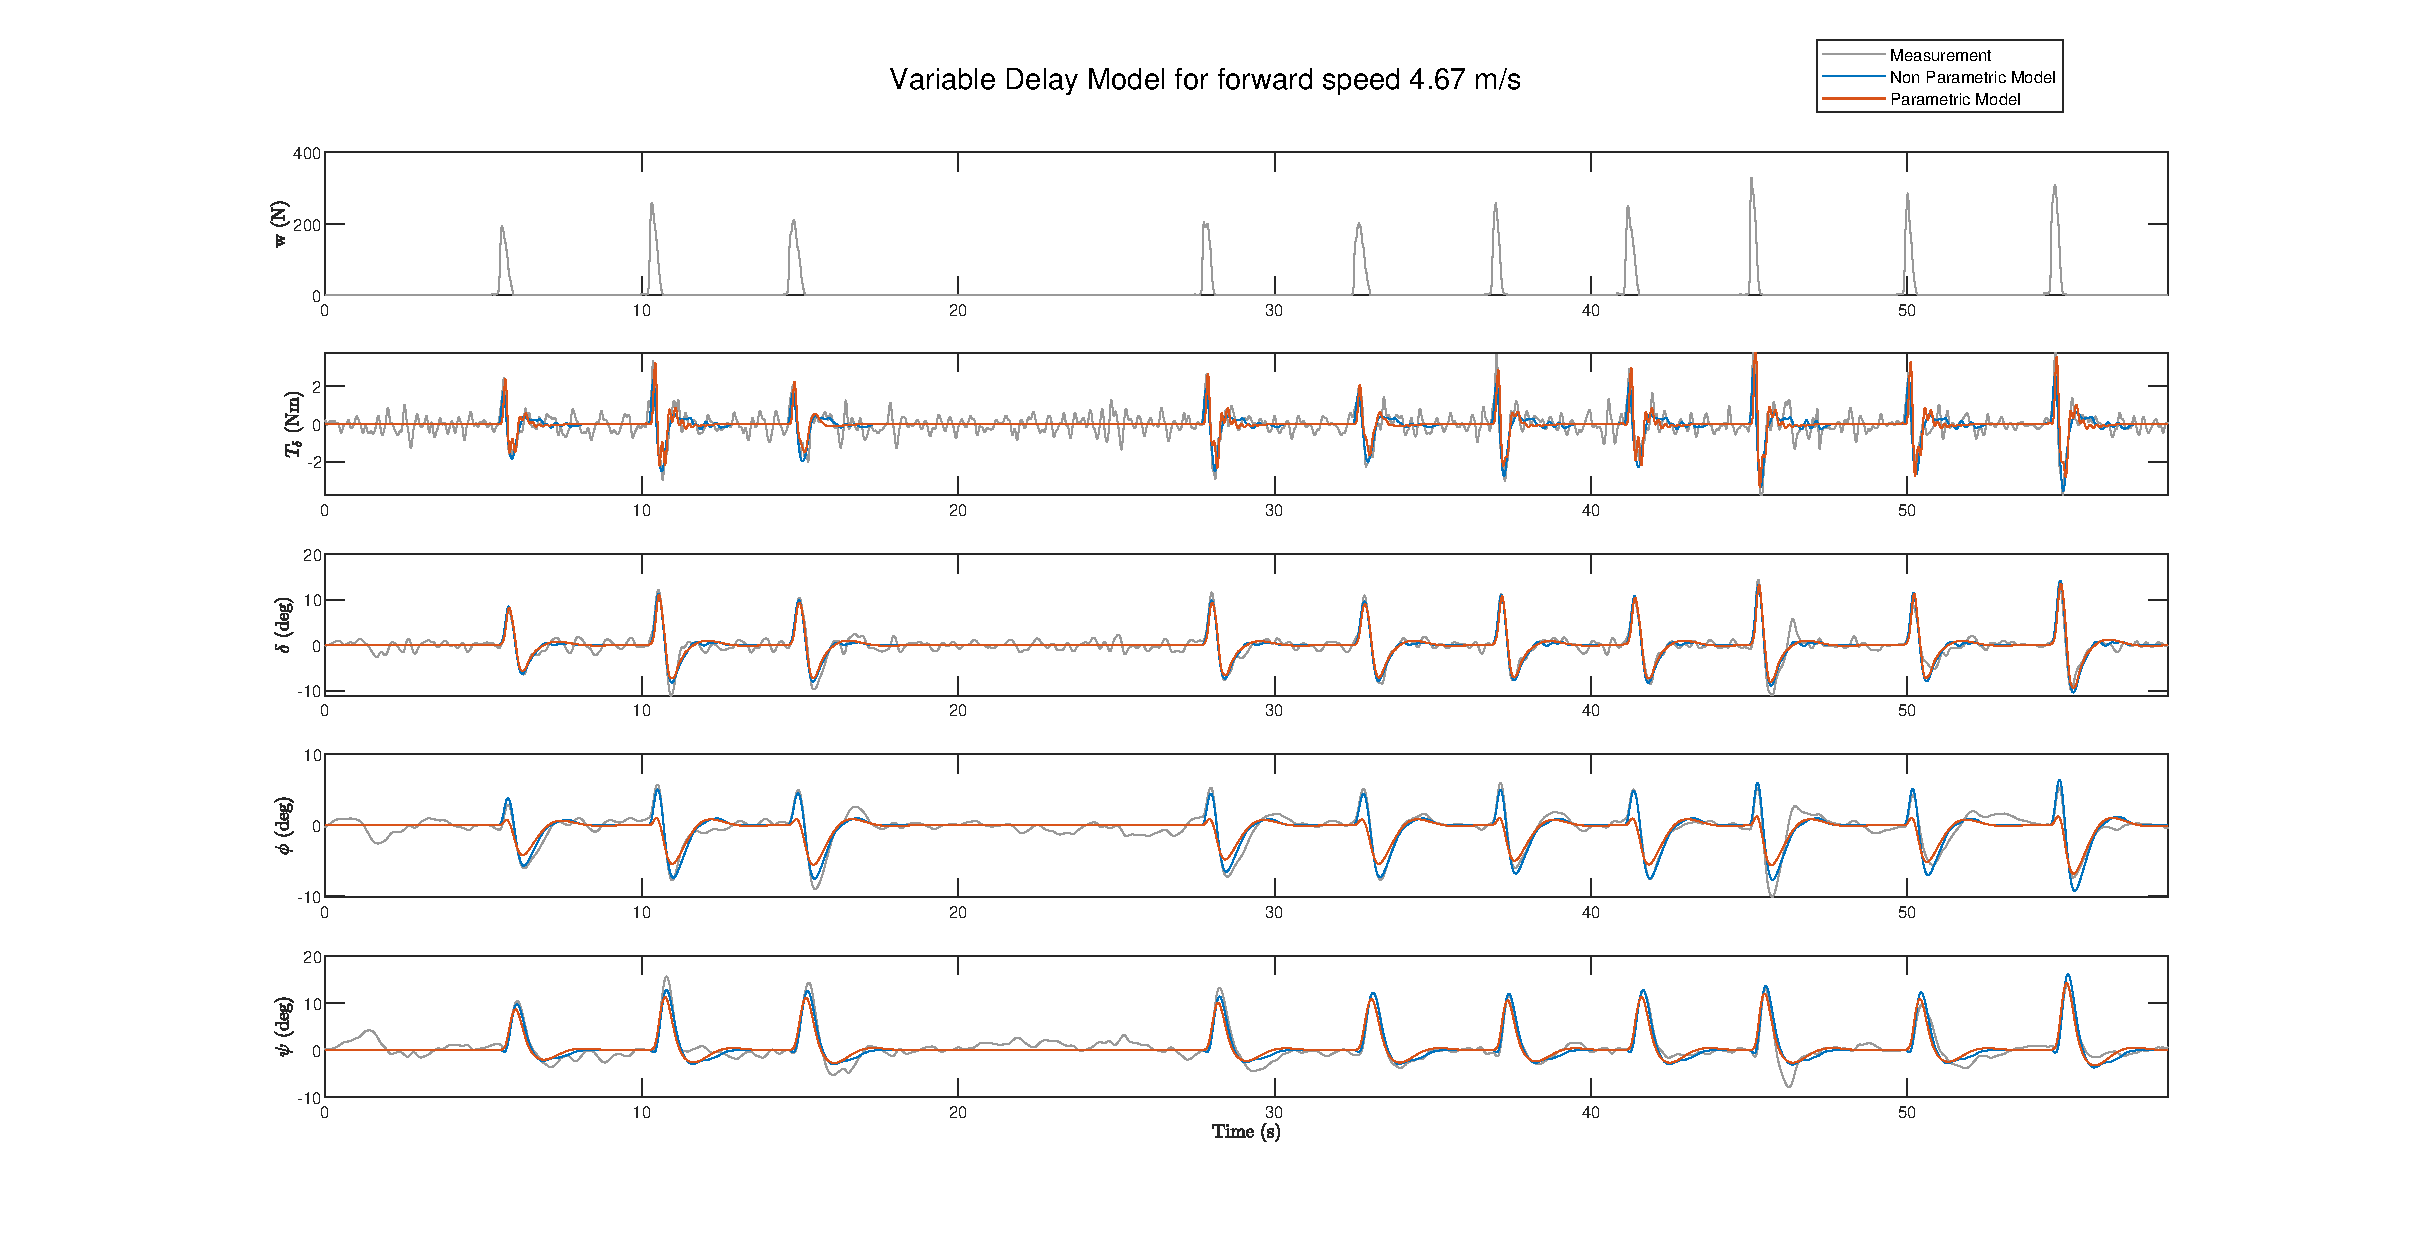
\includegraphics[width=\textwidth]{images/predict_delay_result1.eps}
    \caption{Comparison between variable delay model output, non-parametric model ouput and measured signals for the speed level of 4.67 \si{\meter\per\second} for the case where torque feedback is activated.}
    \label{fig:paper9}
\end{figure}


\begin{figure}[!h]
    \centering
    \captionsetup{justification=centering,margin=2cm}

    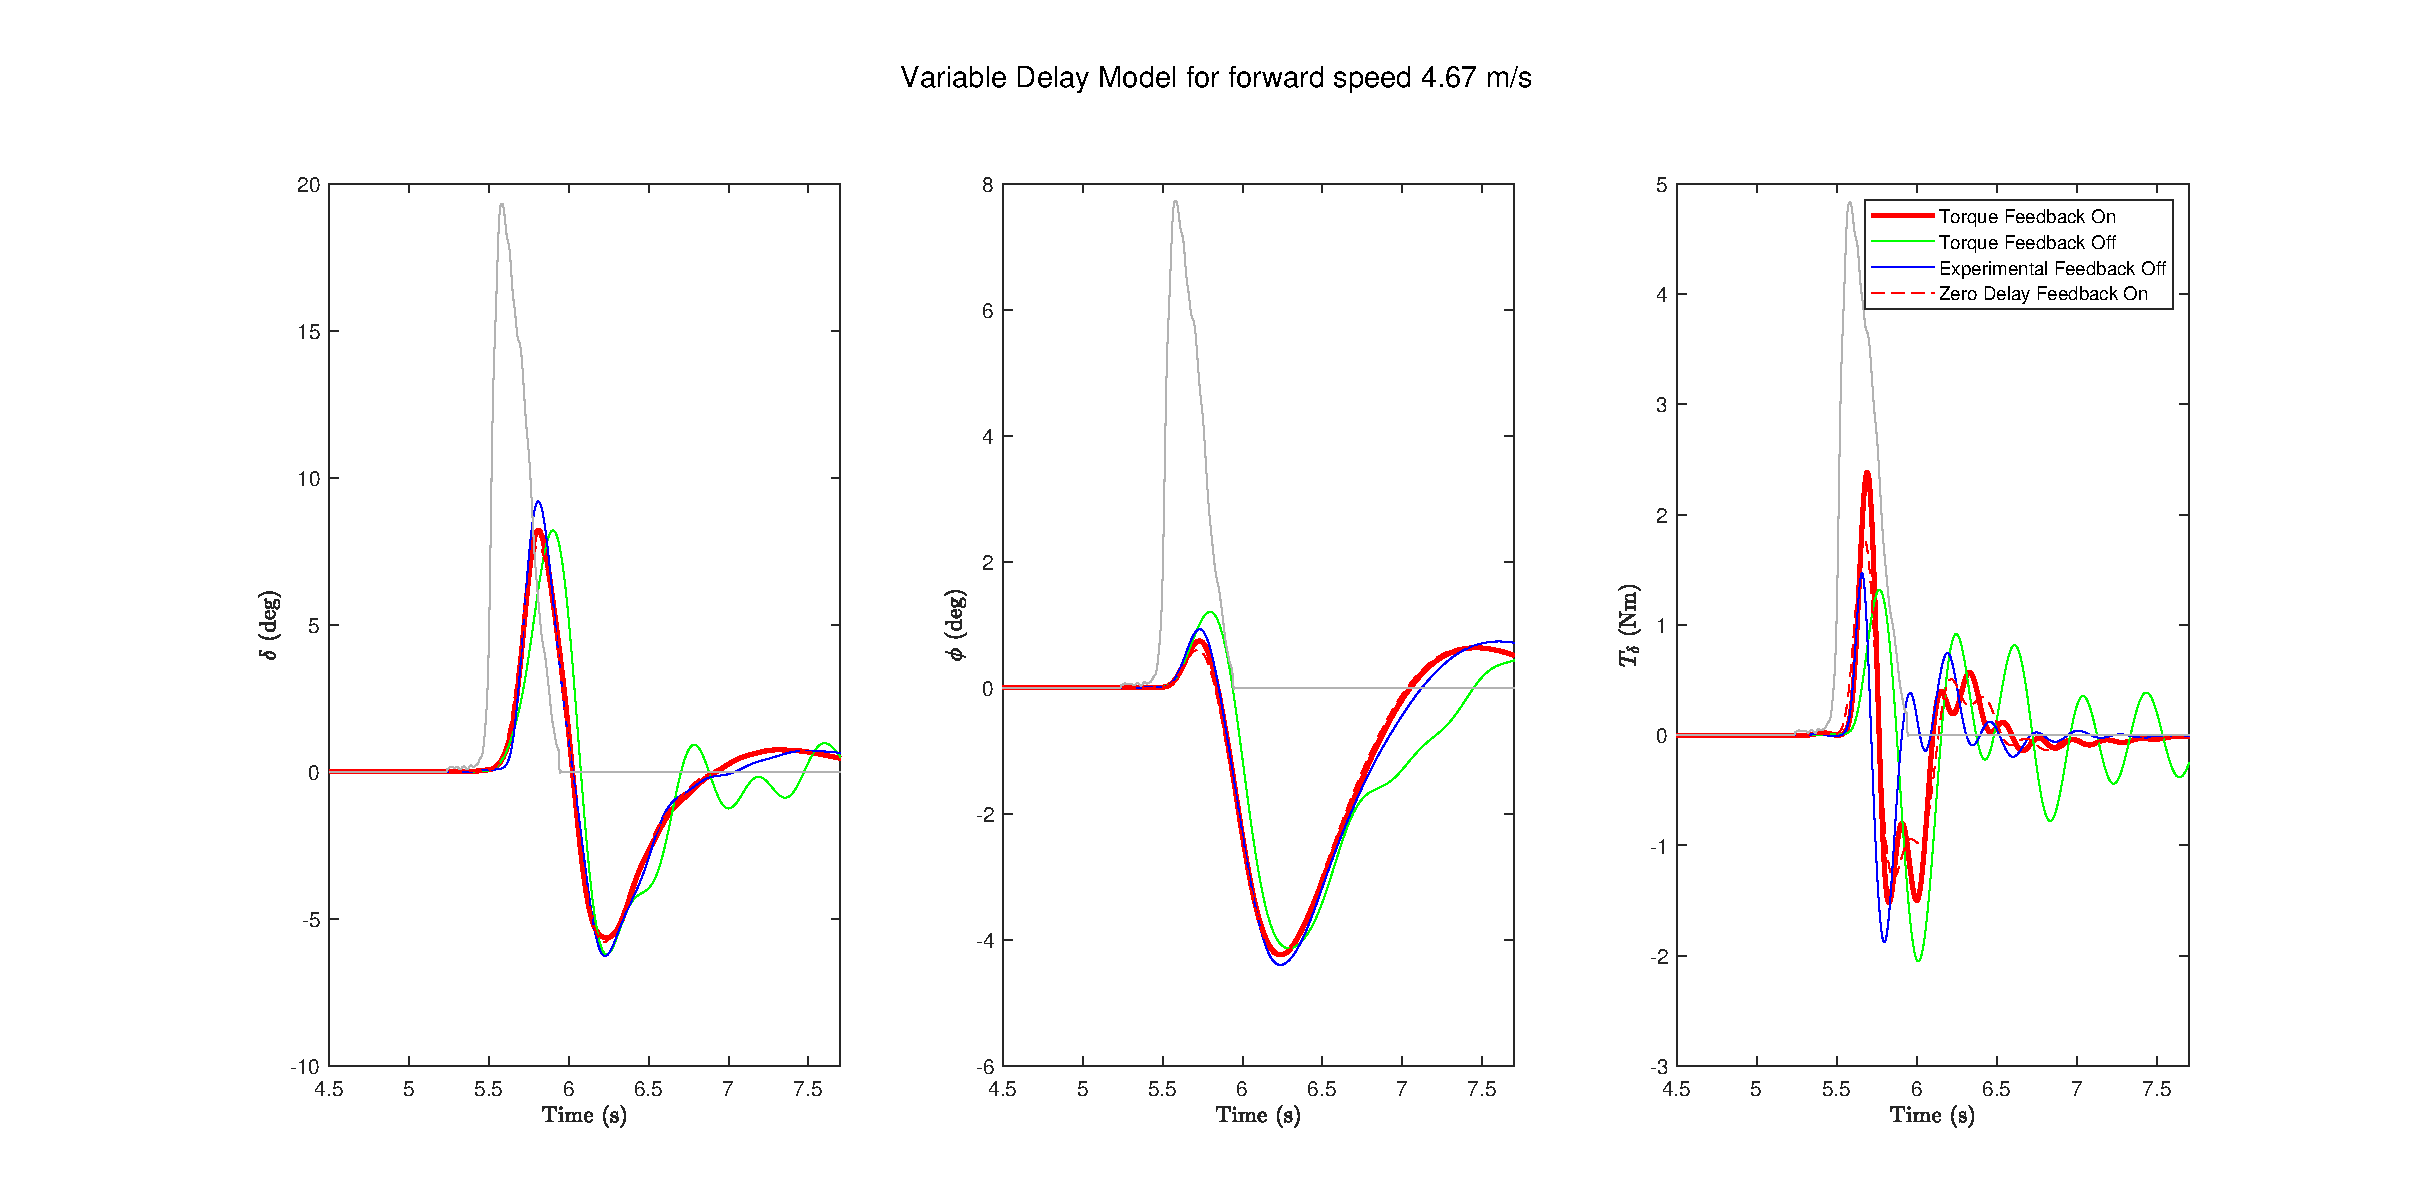
\includegraphics[width=\textwidth]{images/predict_delay_compare2.eps}
    \caption{Steering, roll angles and input rider torque of the variable delay model  compared among torque feedback levels  for the forward speed of 4.67 \si{\meter\per\second}.The red dotted lines is the feedback on case of the zero delay model and is shown for reference. The disturbance signal is not shown  to scale.}
    \label{fig:paper10}
\end{figure}

In \crefrange{fig:results_compare12}{fig:results_compare34}  a complete comparison between rider models for all feedback conditions is presented. The response shown is the result of the first lateral perturbation of each individual run. The zero delay and prediction models exhibit almost identical responses as it was evident from the over 90\% fit achieved. The variable delay model lags behind in both the produced control input and bicycle output, as is expected. Worth noting the lag in the control input of the prediction model in the first few milliseconds after the perturbation. Despite that fact the model compensates and achieves similar ouput as the idealized zero delay case. This is a result of the fact that no matter how good the prediction algorithm is the human has no knowledge of the future so the response from the controller will start after the first state infromation arrives from the feedback pathways which are delayed. The forward model in this case does not help predict the state as it has no information of the external disturbance. 
% Please add the following required packages to your document preamble:
% \usepackage{multirow}





    \begin{figure}
        \centering
        \begin{subfigure}[b]{\textwidth}
            \centering
            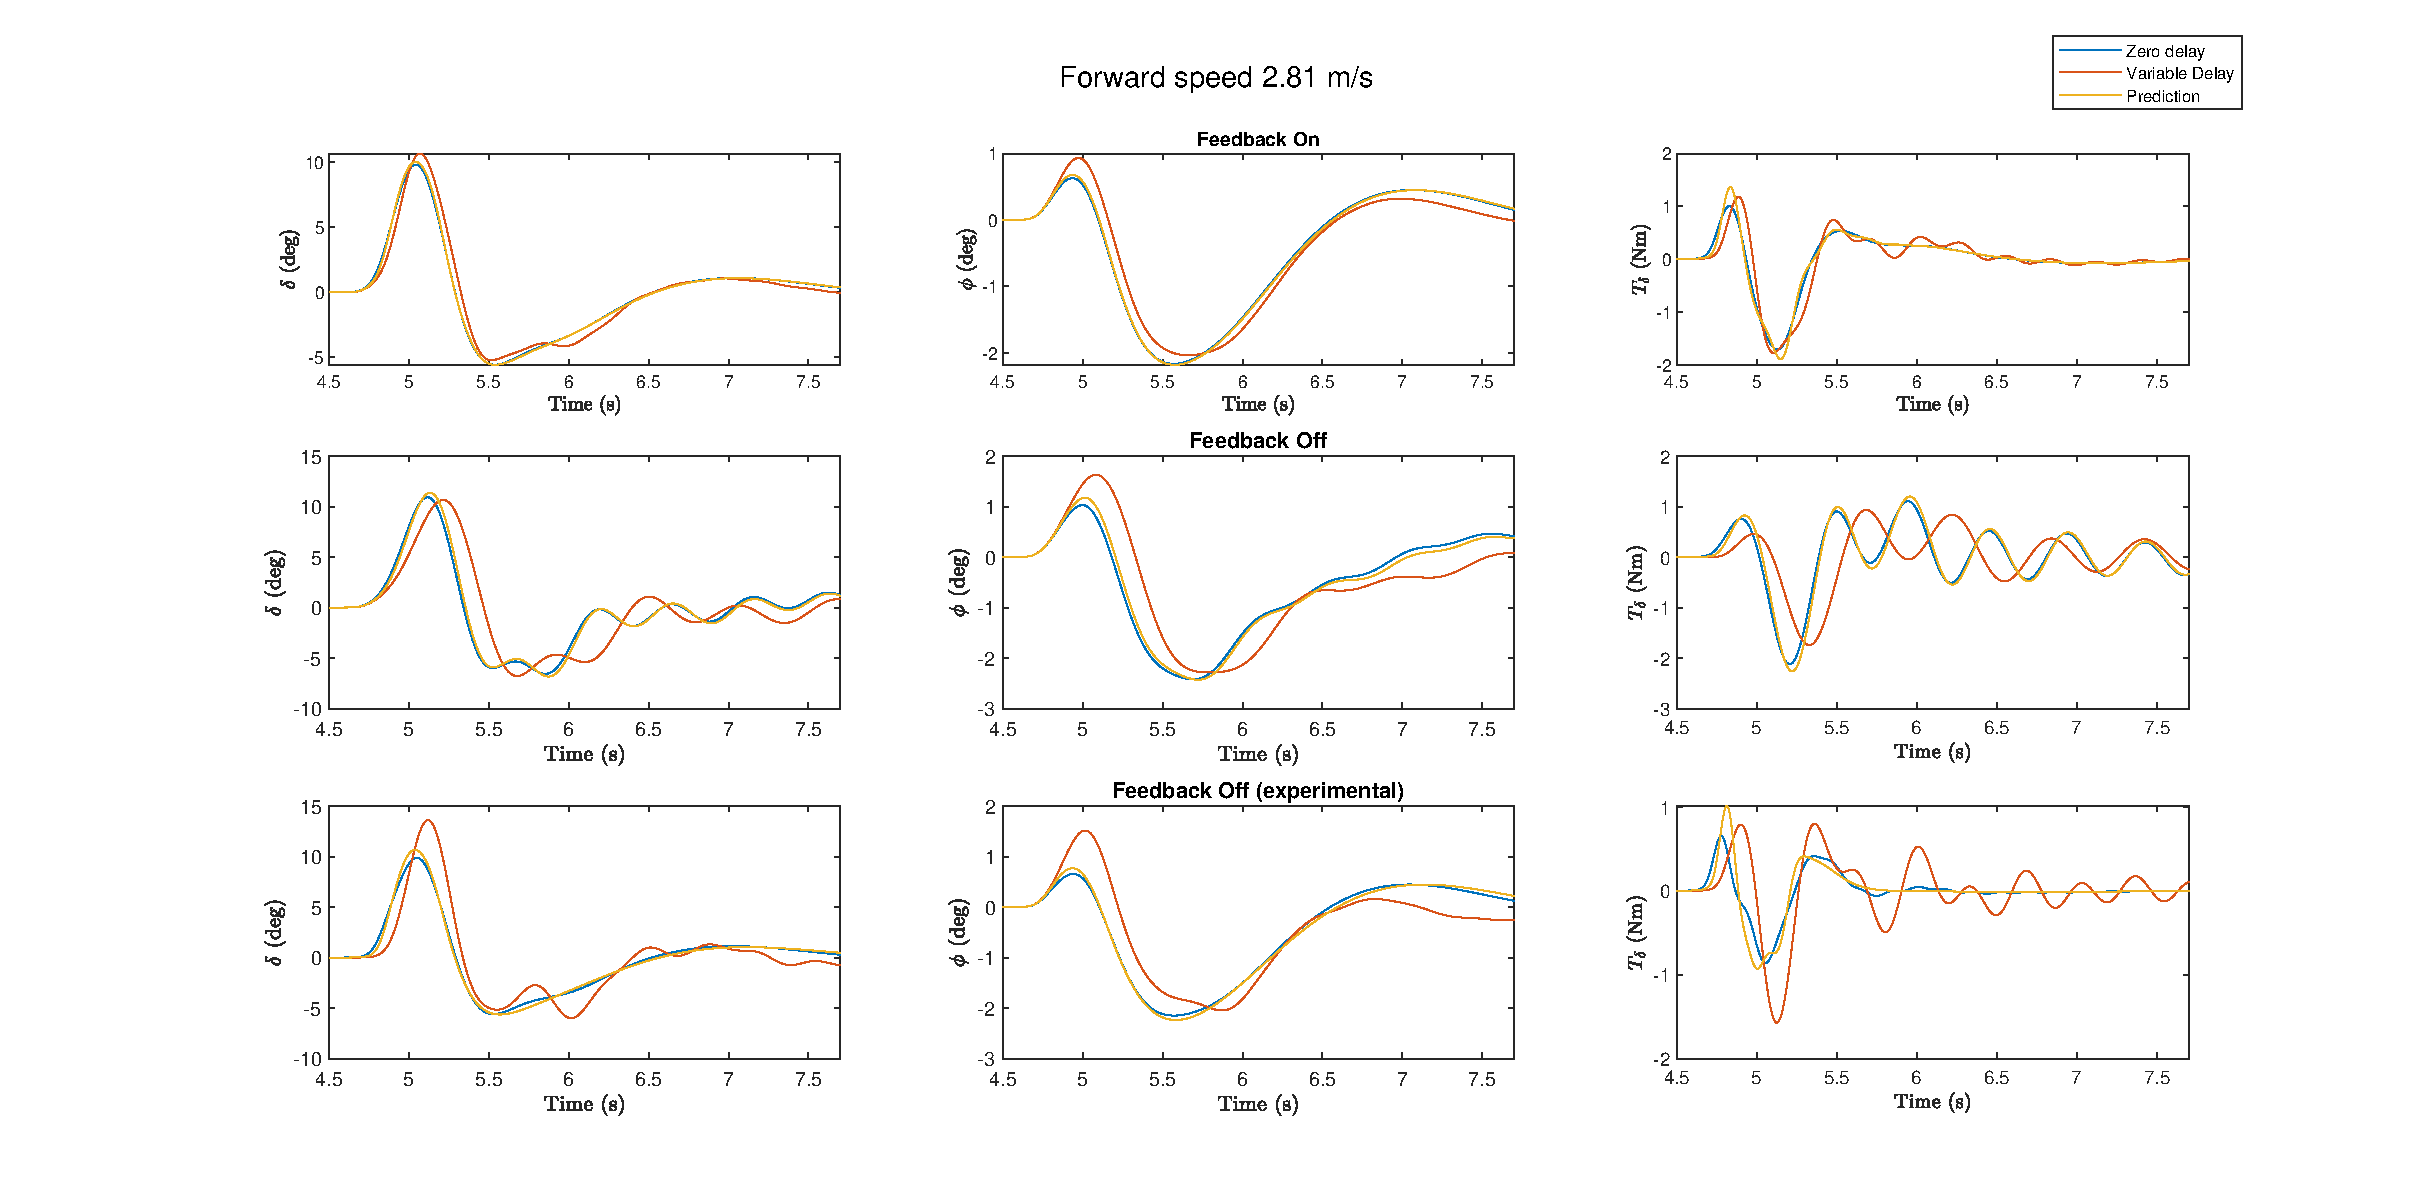
\includegraphics[width=1\linewidth]{images/compare_models.eps}
            \caption{Comparison between the three rider models for forward speed 2.81 \si{\meter\per\second}}
            \label{fig:results_compare1}
        \end{subfigure}
        \begin{subfigure}[b]{\textwidth}
            \centering
            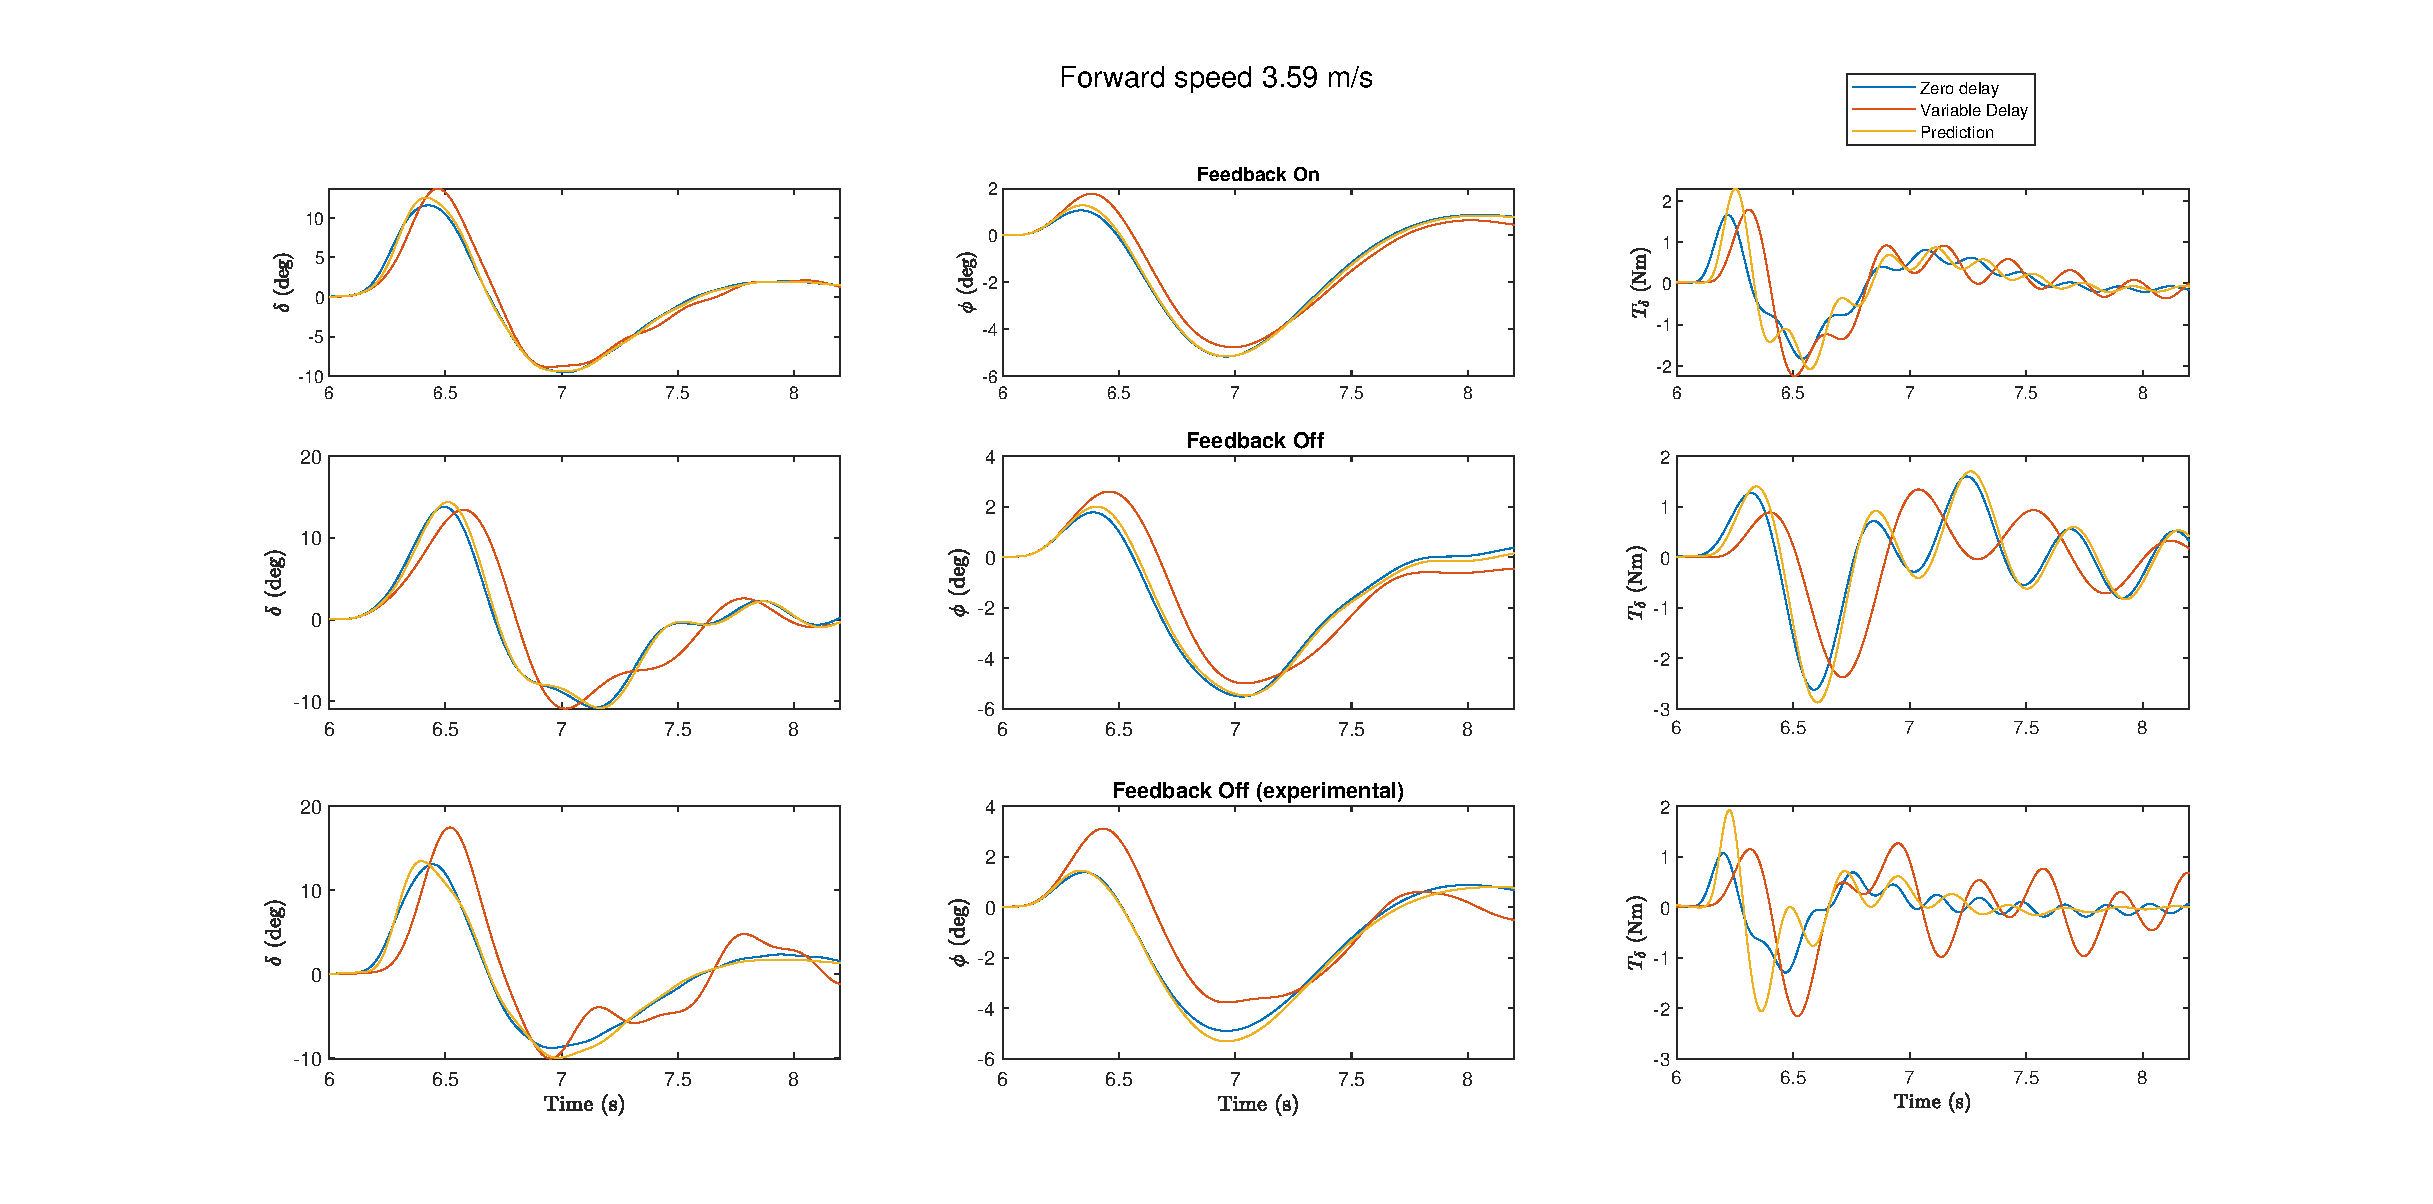
\includegraphics[width=1\linewidth]{images/compare_models2.eps}
            \caption{Comparison between the three rider models for forward speed 3.6 \si{\meter\per\second}}            
            \label{fig:results_compare2}
        \end{subfigure}
        \caption{Steering angle \ensuremath{\delta}, roll angle \ensuremath{\phi} and steering torque \ensuremath{T_\delta} compared among the three rider models implemented for all torque feedback conditions, for the two lowest speed levels.}
        \label{fig:results_compare12}
     \end{figure}



     \begin{figure}
        \centering
        \begin{subfigure}[b]{\textwidth}
            \centering
            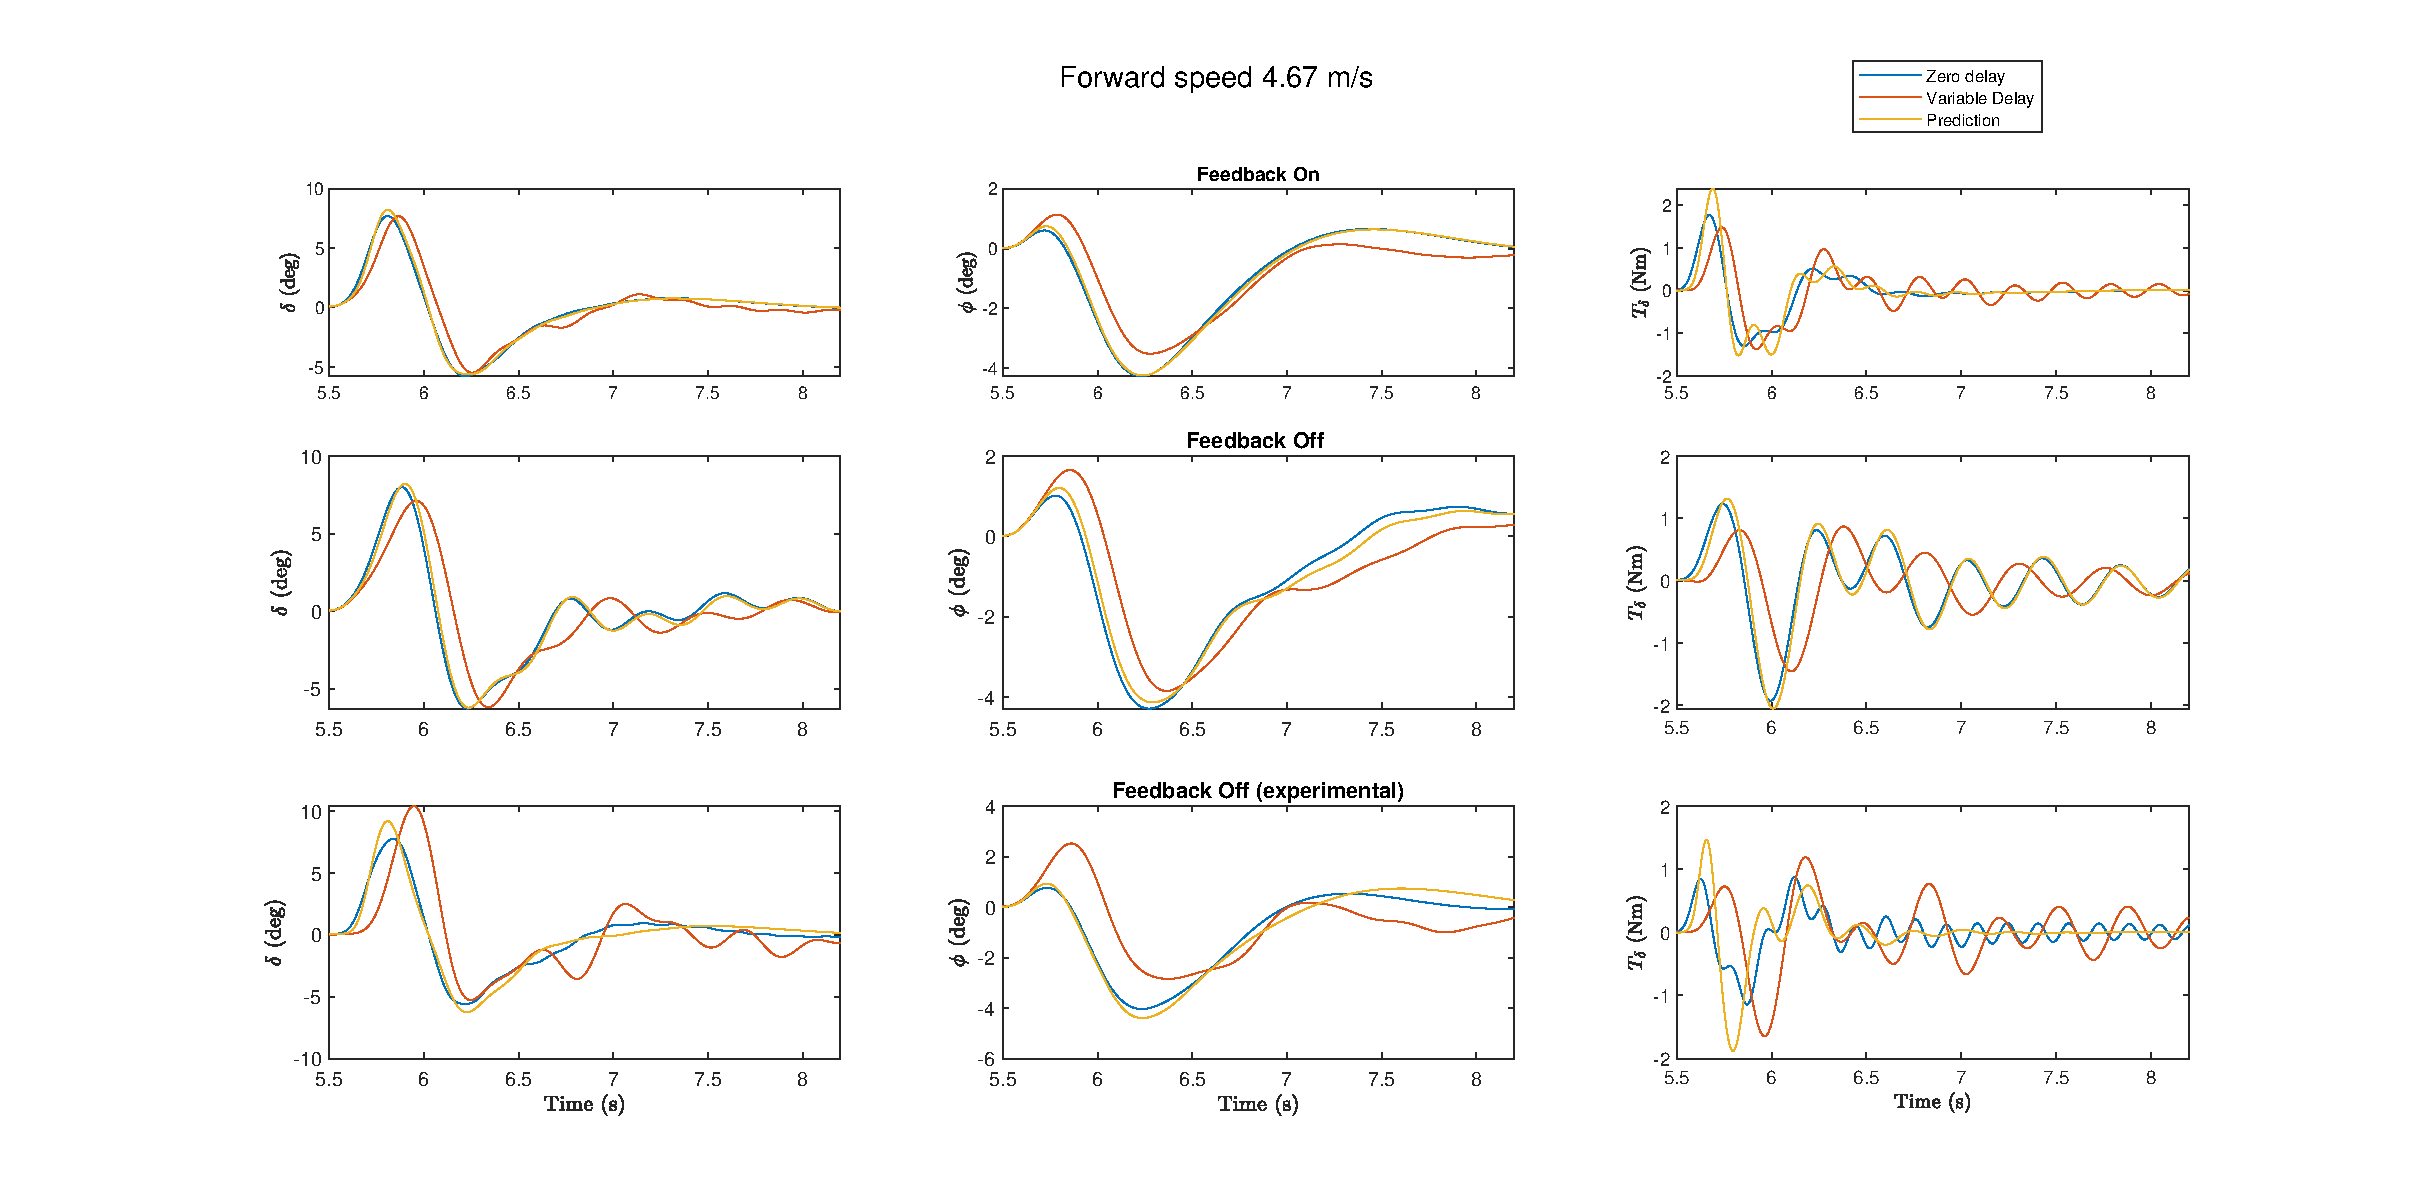
\includegraphics[width=1\linewidth]{images/compare_models3.eps}
            \caption{Comparison between the three rider models for forward speed 4.67 \si{\meter\per\second}}
            \label{fig:results_compare3}
        \end{subfigure}
        \begin{subfigure}[b]{\textwidth}
            \centering
            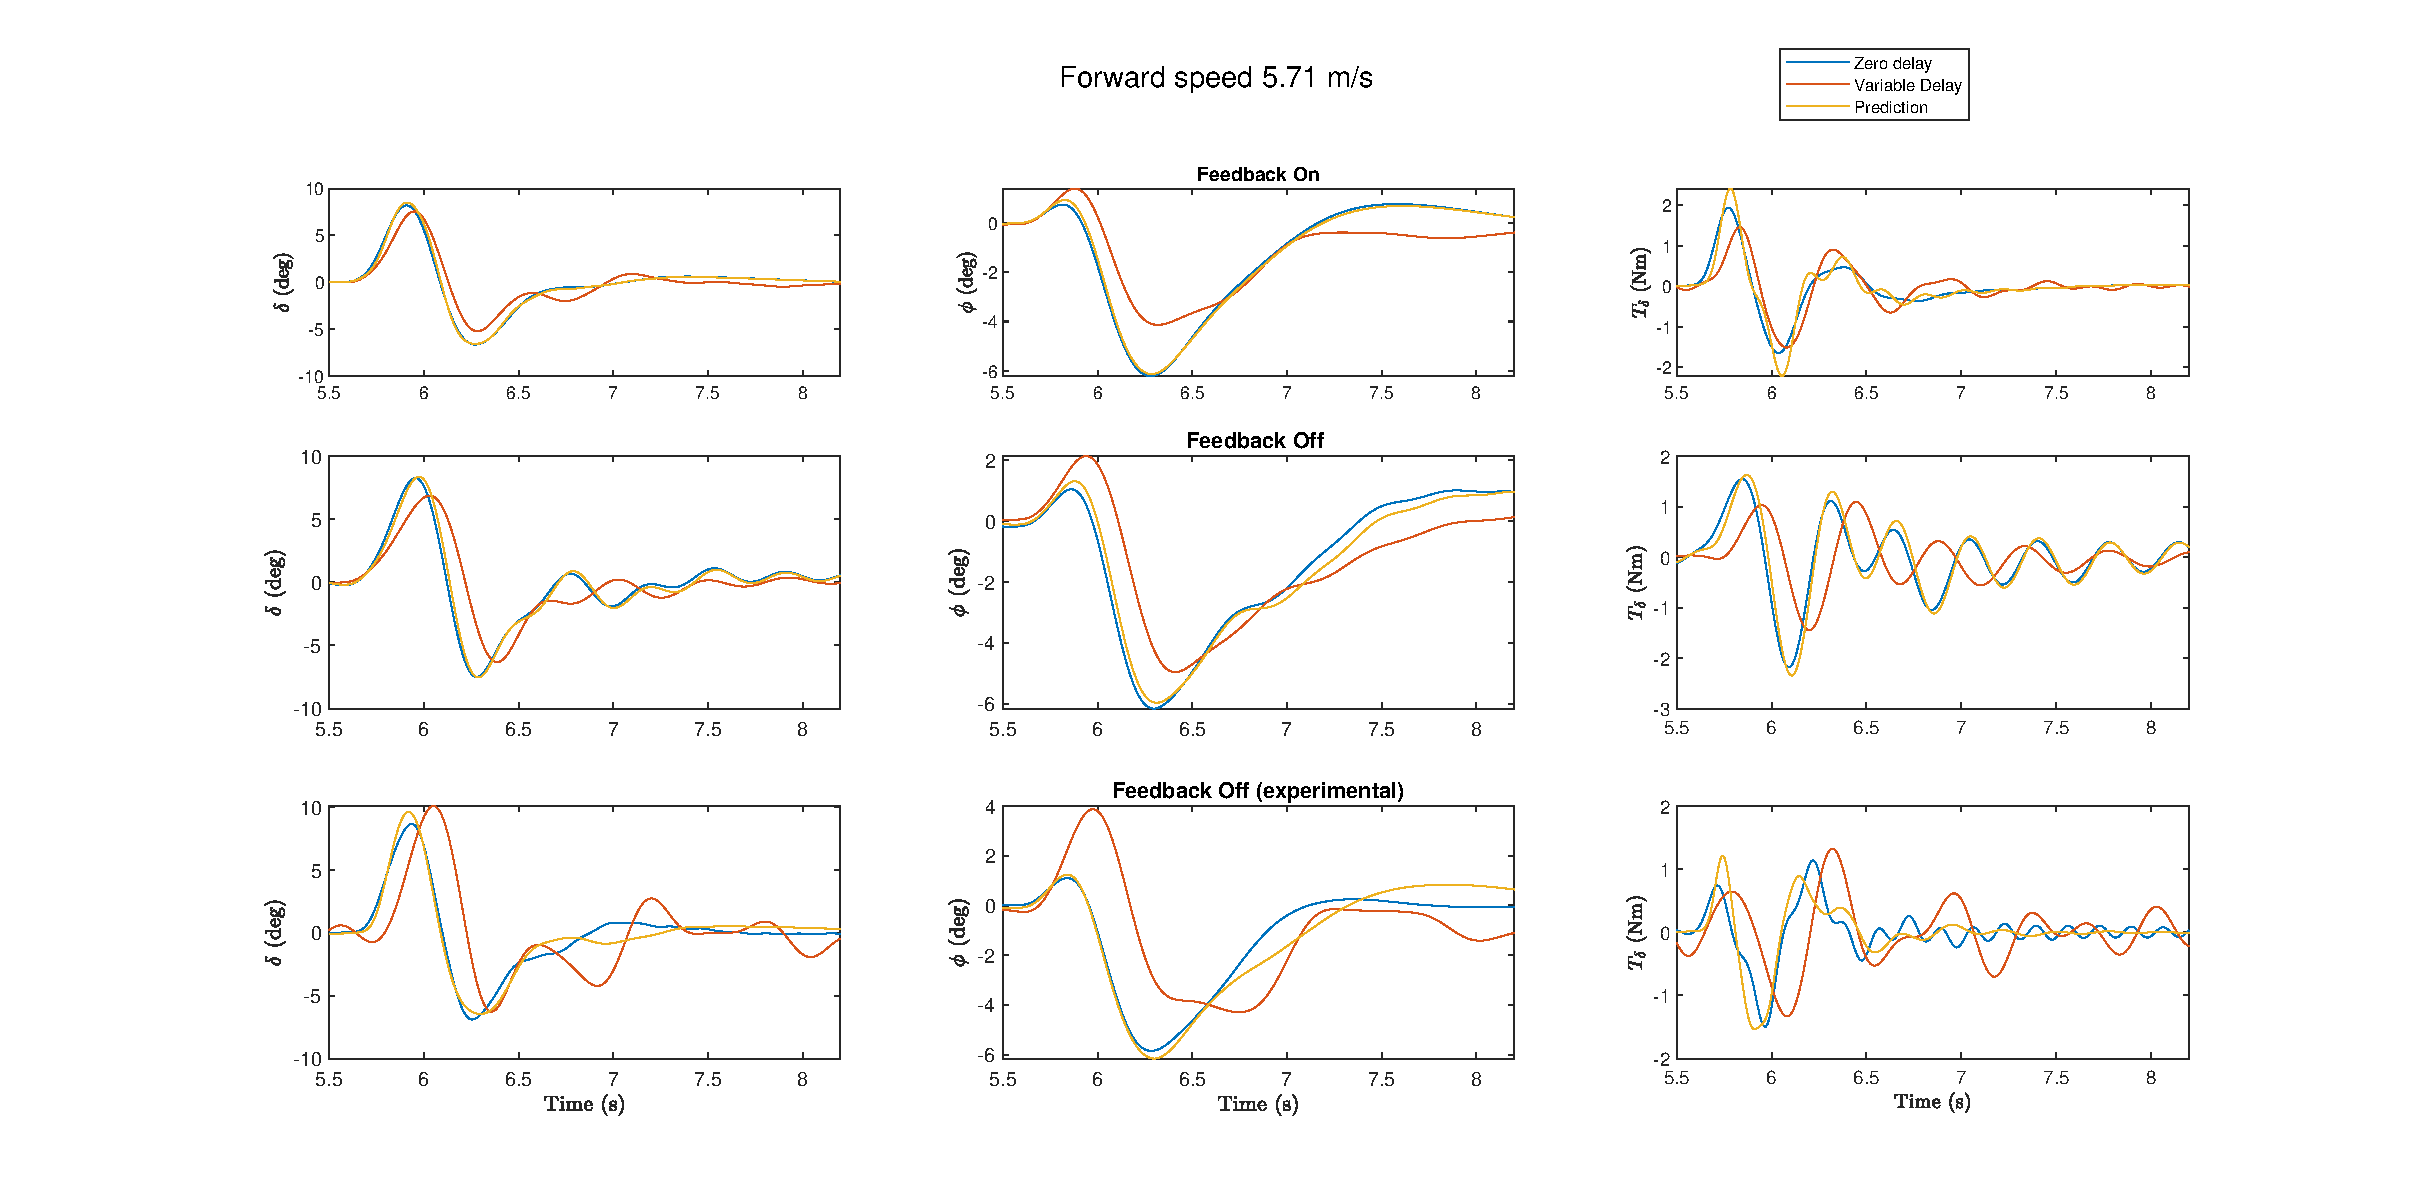
\includegraphics[width=1\linewidth]{images/compare_models4.eps}
            \caption{Comparison between the three rider models for forward speed 5.71 \si{\meter\per\second}}            
            \label{fig:results_compare4}
        \end{subfigure}
        \caption{Steering angle \ensuremath{\delta}, roll angle \ensuremath{\phi} and steering torque \ensuremath{T_\delta} compared among the three rider models implemented for all torque feedback conditions, for the two highest speed levels.}
        \label{fig:results_compare34}
     \end{figure}

% Please add the following required packages to your document preamble:
% \usepackage{multirow}
% Please add the following required packages to your document preamble:
% \usepackage{multirow}
\begin{table}[]
    \caption{ Results for the zero delay model as estimated for the median rider for all speed levels. Results are presented for the three conditions. Feedback on includes torque feedback in the loop while feedback off completely removes it. Feedback off (experimental) is the model response with all loops connected but with the dynamics of the plant modified to simulate the feedback off condition in the experimental setup. The values of the gains are presented as well as their corresponding uncertainty level measured by the index of dispersion \ensuremath{D_i}. Additionally, the variance accounted for of the orientation outputs between parmetric and non parametric signals is also presented. The derivative gains (\ensuremath{K_{\dot{\phi}}},\ensuremath{K_{\dot{\delta}}}) are measured in \si{\kilogram\square\meter\per\square\second} while the proportional gains (\ensuremath{K_{\phi}},\ensuremath{K_{\delta}},\ensuremath{K_{\psi}}) are measured in \si{\kilogram\square\meter\per\second}. The torque feedback gain \ensuremath{K_{T_\delta}} is dimensionless.}
    \begin{tabular}{llcccccc}
    \hline
    Forward Speed                &                       & \multicolumn{2}{l}{Feedback On}                                                                 & \multicolumn{2}{c}{Feedback Off}                                                                & \multicolumn{2}{c}{Feedback Off (experimental)}                                                 \\ \hline
                                 &                       & \multicolumn{1}{l}{\multirow{2}{*}{Value}} & \multicolumn{1}{l}{\multirow{2}{*}{D ($10^{-4}$)}} & \multicolumn{1}{l}{\multirow{2}{*}{Value}} & \multicolumn{1}{l}{\multirow{2}{*}{D ($10^{-4}$)}} & \multicolumn{1}{l}{\multirow{2}{*}{Value}} & \multicolumn{1}{l}{\multirow{2}{*}{D ($10^{-4}$)}} \\
                                 &                       & \multicolumn{1}{l}{}                       & \multicolumn{1}{l}{}                               & \multicolumn{1}{l}{}                       & \multicolumn{1}{l}{}                               & \multicolumn{1}{l}{}                       & \multicolumn{1}{l}{}                               \\ \cline{3-8} 
    2.8 $\si{\meter\per\second}$ & $K_{\dot{\phi}} $     & -77.11                                     & 120.20                                             & -22.46                                     & 1.99                                               & -115.36                                    & 525.96                                             \\
                                 & $K_{\dot{\delta}}$    & 2.27                                       & 4.06                                               & 2.58                                       & 0.09                                               & 8.76                                       & 30.72                                              \\
                                 & $K_{\phi} $           & -164.65                                    & 231.94                                             & -24.5                                      & 13.10                                              & -248.24                                    & 1169.53                                            \\
                                 & $K_\delta $           & 32.65                                      & 56.73                                              & 3.76                                       & 7.47                                               & 29.67                                      & 137.23                                             \\
                                 & $K_\psi $             & -63.16                                     & 106.66                                             & -9.85                                      & 2.84                                               & -93.44                                     & 464.72                                             \\
                                 & $K_{T_\delta}$        & 3.5                                        & 10.52                                              & -                                          & -                                                  & 7.53                                       & 37.73                                              \\ \cline{2-8} 
                                 & $\mathbf{VAF}_\phi$   & \multicolumn{2}{c}{77.78}                                                                       & \multicolumn{2}{c}{82.79}                                                                       & \multicolumn{2}{c}{78.37}                                                                       \\
                                 & $\mathbf{VAF}_\delta$ & \multicolumn{2}{c}{98.34}                                                                       & \multicolumn{2}{c}{79.19}                                                                       & \multicolumn{2}{c}{98.20}                                                                       \\
                                 & $\mathbf{VAF}_\psi$   & \multicolumn{2}{c}{93.44}                                                                       & \multicolumn{2}{c}{93.51}                                                                       & \multicolumn{2}{c}{93.74}                                                                       \\ \hline
                                 &                       & \multicolumn{1}{l}{\multirow{2}{*}{Value}} & \multicolumn{1}{l}{\multirow{2}{*}{D ($10^{-4}$)}} & \multicolumn{1}{l}{\multirow{2}{*}{Value}} & \multicolumn{1}{l}{\multirow{2}{*}{D ($10^{-4}$)}} & \multicolumn{1}{l}{\multirow{2}{*}{Value}} & \multicolumn{1}{l}{\multirow{2}{*}{D ($10^{-4}$)}} \\
                                 &                       & \multicolumn{1}{l}{}                       & \multicolumn{1}{l}{}                               & \multicolumn{1}{l}{}                       & \multicolumn{1}{l}{}                               & \multicolumn{1}{l}{}                       & \multicolumn{1}{l}{}                               \\ \cline{3-8} 
    3.6 $\si{\meter\per\second}$ & $K_{\dot{\phi}} $     & -109.94                                    & 237.50                                             & -21.30                                     & 2.76                                               & -78.28                                     & 29.13                                              \\
                                 & $K_{\dot{\delta}}$    & 8.22                                       & 15.88                                              & 3.30                                       & 0.20                                               & 9.09                                       & 2.37                                               \\
                                 & $K_{\phi} $           & -248.47                                    & 539.80                                             & -34.64                                     & 17.73                                              & -229.14                                    & 163.22                                             \\
                                 & $K_\delta $           & 50.78                                      & 110.81                                             & 6.48                                       & 11.05                                              & 53.16                                      & 45.93                                              \\
                                 & $K_\psi $             & -132.13                                    & 305.58                                             & -17.74                                     & 6.80                                               & -103.75                                    & 57.57                                              \\
                                 & $K_{T_\delta}$        & 4.52                                       & 12.65                                              & -                                          & -                                                  & 6.89                                       & 2.84                                               \\ \cline{2-8} 
                                 & $\mathbf{VAF}_\phi$   & \multicolumn{2}{c}{79.92}                                                                       & \multicolumn{2}{c}{85.93}                                                                       & \multicolumn{2}{c}{80.89}                                                                       \\
                                 & $\mathbf{VAF}_\delta$ & \multicolumn{2}{c}{98.83}                                                                       & \multicolumn{2}{c}{86.40}                                                                       & \multicolumn{2}{c}{97.08}                                                                       \\
                                 & $\mathbf{VAF}_\psi$   & \multicolumn{2}{c}{95.33}                                                                       & \multicolumn{2}{c}{97.95}                                                                       & \multicolumn{2}{c}{95.15}                                                                       \\ \hline
                                 &                       & \multicolumn{1}{l}{\multirow{2}{*}{Value}} & \multicolumn{1}{l}{\multirow{2}{*}{D ($10^{-4}$)}} & \multicolumn{1}{l}{\multirow{2}{*}{Value}} & \multicolumn{1}{l}{\multirow{2}{*}{D ($10^{-4}$)}} & \multicolumn{1}{l}{\multirow{2}{*}{Value}} & \multicolumn{1}{l}{\multirow{2}{*}{D ($10^{-4}$)}} \\
                                 &                       & \multicolumn{1}{l}{}                       & \multicolumn{1}{l}{}                               & \multicolumn{1}{l}{}                       & \multicolumn{1}{l}{}                               & \multicolumn{1}{l}{}                       & \multicolumn{1}{l}{}                               \\ \cline{3-8} 
    4.7 $\si{\meter\per\second}$ & $K_{\dot{\phi}} $     & -92.50                                     & 127.37                                             & -27.29                                     & 5.88                                               & -102.63                                    & 17.14                                              \\
                                 & $K_{\dot{\delta}}$    & 4.81                                       & 16.11                                              & 4.25                                       & 0.73                                               & 11.24                                      & 0.91                                               \\
                                 & $K_{\phi} $           & -183.03                                    & 336.73                                             & -38.17                                     & 22.30                                              & -249.74                                    & 137.13                                             \\
                                 & $K_\delta $           & 22.57                                      & 127.32                                             & 2.65                                       & 92.80                                              & 63.36                                      & 49.43                                              \\
                                 & $K_\psi $             & -165.42                                    & 266.33                                             & -33.78                                     & 13.73                                              & -188.67                                    & 65.25                                              \\
                                 & $K_{T_\delta}$        & 3.42                                       & 10.37                                              & -                                          & -                                                  & 8.98                                       & 0.17                                               \\ \cline{2-8} 
                                 & $\mathbf{VAF}_\phi$   & \multicolumn{2}{c}{77.03}                                                                       & \multicolumn{2}{c}{83.06}                                                                       & \multicolumn{2}{c}{78.60}                                                                       \\
                                 & $\mathbf{VAF}_\delta$ & \multicolumn{2}{c}{97.57}                                                                       & \multicolumn{2}{c}{80.27}                                                                       & \multicolumn{2}{c}{95.57}                                                                       \\
                                 & $\mathbf{VAF}_\psi$   & \multicolumn{2}{c}{91.41}                                                                       & \multicolumn{2}{c}{97.03}                                                                       & \multicolumn{2}{c}{92.48}                                                                       \\ \hline
                                 &                       & \multicolumn{1}{l}{\multirow{2}{*}{Value}} & \multicolumn{1}{l}{\multirow{2}{*}{D ($10^{-4}$)}} & \multicolumn{1}{l}{\multirow{2}{*}{Value}} & \multicolumn{1}{l}{\multirow{2}{*}{D ($10^{-4}$)}} & \multicolumn{1}{l}{\multirow{2}{*}{Value}} & \multicolumn{1}{l}{\multirow{2}{*}{D ($10^{-4}$)}} \\
                                 &                       & \multicolumn{1}{l}{}                       & \multicolumn{1}{l}{}                               & \multicolumn{1}{l}{}                       & \multicolumn{1}{l}{}                               & \multicolumn{1}{l}{}                       & \multicolumn{1}{l}{}                               \\ \cline{3-8} 
    5.7 $\si{\meter\per\second}$ & $K_{\dot{\phi}} $     & -83.90                                     & 116.05                                             & -31.12                                     & 6.02                                               & -76.30                                     & 16.94                                              \\
                                 & $K_{\dot{\delta}}$    & 5.83                                       & 11.89                                              & 5.58                                       & 0.92                                               & 10.91                                      & 1.00                                               \\
                                 & $K_{\phi} $           & -166.08                                    & 271.62                                             & -43.64                                     & 19.67                                              & -208.33                                    & 143.84                                             \\
                                 & $K_\delta $           & 14.85                                      & 14.29                                              & 1.14                                       & 385.00                                             & 79.44                                      & 45.25                                              \\
                                 & $K_\psi $             & -186.77                                    & 308.69                                             & -49.82                                     & 13.63                                              & -176.96                                    & 86.27                                              \\
                                 & $K_{T_\delta}$        & 3.24                                       & 11.10                                              & -                                          & -                                                  & 8.45                                       & 0.74                                               \\ \cline{2-8} 
                                 & $\mathbf{VAF}_\phi$   & \multicolumn{2}{c}{79.17}                                                                       & \multicolumn{2}{c}{84.03}                                                                       & \multicolumn{2}{c}{80.30}                                                                       \\
                                 & $\mathbf{VAF}_\delta$ & \multicolumn{2}{c}{97.51}                                                                       & \multicolumn{2}{c}{84.09}                                                                       & \multicolumn{2}{c}{94.71}                                                                       \\
                                 & $\mathbf{VAF}_\psi$   & \multicolumn{2}{c}{90.97}                                                                       & \multicolumn{2}{c}{96.41}                                                                       & \multicolumn{2}{c}{91.56}                                                                      
    \end{tabular}
    \label{tb:no_delay}
    \end{table}
\begin{table}[]
    \caption{ Results for the variable delay model as estimated for the median rider for all speed levels. Results are presented for the three conditions. Feedback on includes torque feedback in the loop while feedback off completely removes it. Feedback off (experimental) is the model response with all loops connected but with the dynamics of the plant modified to simulate the feedback off condition in the experimental setup. The values of the gains are presented as well as their corresponding uncertainty level measured by the index of dispersion \ensuremath{D_i} (dimensionless). Additionally, the variance accounted for of the orientation outputs between parmetric and non parametric signals is also presented. The derivative gains (\ensuremath{K_{\dot{\phi}}},\ensuremath{K_{\dot{\delta}}}) are measured in \si{\kilogram\square\meter\per\square\second} while the proportional gains (\ensuremath{K_{\phi}},\ensuremath{K_{\delta}},\ensuremath{K_{\psi}}) are measured in \si{\kilogram\square\meter\per\second}. The torque feedback gain \ensuremath{K_{T_\delta}} is dimensionless.}
    \begin{tabular}{llcccccc}
    \hline
    Forward Speed                &                       & \multicolumn{2}{l}{Feedback On}                                                                 & \multicolumn{2}{c}{Feedback Off}                                                                & \multicolumn{2}{c}{Feedback Off (experimental)}                                                 \\ \hline
                                 &                       & \multicolumn{1}{l}{\multirow{2}{*}{Value}} & \multicolumn{1}{l}{\multirow{2}{*}{D ($10^{-4}$)}} & \multicolumn{1}{l}{\multirow{2}{*}{Value}} & \multicolumn{1}{l}{\multirow{2}{*}{D ($10^{-4}$)}} & \multicolumn{1}{l}{\multirow{2}{*}{Value}} & \multicolumn{1}{l}{\multirow{2}{*}{D ($10^{-4}$)}} \\
                                 &                       & \multicolumn{1}{l}{}                       & \multicolumn{1}{l}{}                               & \multicolumn{1}{l}{}                       & \multicolumn{1}{l}{}                               & \multicolumn{1}{l}{}                       & \multicolumn{1}{l}{}                               \\ \cline{3-8} 
    2.8 $\si{\meter\per\second}$ & $K_{\dot{\phi}} $     & -68.53                                     & 10.28                                              & -14.93                                     & 2.10                                               & -28.19                                     & 3.48                                               \\
                                 & $K_{\dot{\delta}}$    & 2.09                                       & 2.54                                               & 2.30                                       & 0.24                                               & 2.65                                       & 0.05                                               \\
                                 & $K_{\phi} $           & -146.29                                    & 75.99                                              & -16.98                                     & 14.54                                              & -79.20                                     & 48.69                                              \\
                                 & $K_\delta $           & 22.18                                      & 20.18                                              & 4.62                                       & 4.98                                               & 10.51                                      & 9.16                                               \\
                                 & $K_\psi $             & -40.34                                     & 12.73                                              & -3.78                                      & 5.16                                               & -14.53                                     & 6.54                                               \\
                                 & $K_{T_\delta}$        & 3.52                                       & 1.48                                               & -                                          & -                                                  & 2.59                                       & 0.23                                               \\ \cline{2-8} 
                                 & $\mathbf{VAF}_\phi$   & \multicolumn{2}{c}{81.15}                                                                       & \multicolumn{2}{c}{69.61}                                                                       & \multicolumn{2}{c}{80.01}                                                                       \\
                                 & $\mathbf{VAF}_\delta$ & \multicolumn{2}{c}{93.43}                                                                       & \multicolumn{2}{c}{23.34}                                                                       & \multicolumn{2}{c}{66.84}                                                                       \\
                                 & $\mathbf{VAF}_\psi$   & \multicolumn{2}{c}{93.78}                                                                       & \multicolumn{2}{c}{69.67}                                                                       & \multicolumn{2}{c}{83.30}                                                                       \\ \hline
                                 &                       & \multicolumn{1}{l}{\multirow{2}{*}{Value}} & \multicolumn{1}{l}{\multirow{2}{*}{D ($10^{-4}$)}} & \multicolumn{1}{l}{\multirow{2}{*}{Value}} & \multicolumn{1}{l}{\multirow{2}{*}{D ($10^{-4}$)}} & \multicolumn{1}{l}{\multirow{2}{*}{Value}} & \multicolumn{1}{l}{\multirow{2}{*}{D ($10^{-4}$)}} \\
                                 &                       & \multicolumn{1}{l}{}                       & \multicolumn{1}{l}{}                               & \multicolumn{1}{l}{}                       & \multicolumn{1}{l}{}                               & \multicolumn{1}{l}{}                       & \multicolumn{1}{l}{}                               \\ \cline{3-8} 
    3.6 $\si{\meter\per\second}$ & $K_{\dot{\phi}} $     & -51.02                                     & 16.35                                              & -15.40                                     & 4.81                                               & -21.25                                     & 5.60                                               \\
                                 & $K_{\dot{\delta}}$    & 2.50                                       & 7.26                                               & 2.81                                       & 0.71                                               & 2.79                                       & 0.09                                               \\
                                 & $K_{\phi} $           & -120.51                                    & 87.65                                              & -22.82                                     & 24.13                                              & -76.41                                     & 63.12                                              \\
                                 & $K_\delta $           & 16.58                                      & 38.96                                              & 3.94                                       & 23.42                                              & 17.14                                      & 12.36                                              \\
                                 & $K_\psi $             & -43.06                                     & 27.15                                              & -7.37                                      & 16.00                                              & -13.30                                     & 14.25                                              \\
                                 & $K_{T_\delta}$        & 3.42                                       & 1.35                                               & -                                          & -                                                  & 3.09                                       & 0.14                                               \\ \cline{2-8} 
                                 & $\mathbf{VAF}_\phi$   & \multicolumn{2}{c}{82.85}                                                                       & \multicolumn{2}{c}{79.48}                                                                       & \multicolumn{2}{c}{73.14}                                                                       \\
                                 & $\mathbf{VAF}_\delta$ & \multicolumn{2}{c}{91.63}                                                                       & \multicolumn{2}{c}{53.29}                                                                       & \multicolumn{2}{c}{52.83}                                                                       \\
                                 & $\mathbf{VAF}_\psi$   & \multicolumn{2}{c}{95.10}                                                                       & \multicolumn{2}{c}{84.88}                                                                       & \multicolumn{2}{c}{71.58}                                                                       \\ \hline
                                 &                       & \multicolumn{1}{l}{\multirow{2}{*}{Value}} & \multicolumn{1}{l}{\multirow{2}{*}{D ($10^{-4}$)}} & \multicolumn{1}{l}{\multirow{2}{*}{Value}} & \multicolumn{1}{l}{\multirow{2}{*}{D ($10^{-4}$)}} & \multicolumn{1}{l}{\multirow{2}{*}{Value}} & \multicolumn{1}{l}{\multirow{2}{*}{D ($10^{-4}$)}} \\
                                 &                       & \multicolumn{1}{l}{}                       & \multicolumn{1}{l}{}                               & \multicolumn{1}{l}{}                       & \multicolumn{1}{l}{}                               & \multicolumn{1}{l}{}                       & \multicolumn{1}{l}{}                               \\ \cline{3-8} 
    4.7 $\si{\meter\per\second}$ & $K_{\dot{\phi}} $     & -51.78                                     & 21.61                                              & -19.26                                     & 235.55                                             & -14.88                                     & 4.65                                               \\
                                 & $K_{\dot{\delta}}$    & 2.75                                       & 7.09                                               & 4.42                                       & 85.20                                              & 3.04                                       & 0.13                                               \\
                                 & $K_{\phi} $           & -136.22                                    & 150.61                                             & -27.02                                     & 33.76                                              & -48.91                                     & 65.70                                              \\
                                 & $K_\delta $           & 3.21                                       & 428.40                                             & 0.01                                       & 345508.59                                          & 16.01                                      & 15.78                                              \\
                                 & $K_\psi $             & -64.43                                     & 49.44                                              & -14.29                                     & 243.82                                             & -10.82                                     & 15.45                                              \\
                                 & $K_{T_\delta}$        & 3.70                                       & 1.51                                               & -                                          & -                                                  & 2.61                                       & 0.24                                               \\ \cline{2-8} 
                                 & $\mathbf{VAF}_\phi$   & \multicolumn{2}{c}{77.86}                                                                       & \multicolumn{2}{c}{71.14}                                                                       & \multicolumn{2}{c}{63.73}                                                                       \\
                                 & $\mathbf{VAF}_\delta$ & \multicolumn{2}{c}{81.63}                                                                       & \multicolumn{2}{c}{36.19}                                                                       & \multicolumn{2}{c}{15.61}                                                                       \\
                                 & $\mathbf{VAF}_\psi$   & \multicolumn{2}{c}{90.32}                                                                       & \multicolumn{2}{c}{80.57}                                                                       & \multicolumn{2}{c}{55.71}                                                                       \\ \hline
                                 &                       & \multicolumn{1}{l}{\multirow{2}{*}{Value}} & \multicolumn{1}{l}{\multirow{2}{*}{D ($10^{-4}$)}} & \multicolumn{1}{l}{\multirow{2}{*}{Value}} & \multicolumn{1}{l}{\multirow{2}{*}{D ($10^{-4}$)}} & \multicolumn{1}{l}{\multirow{2}{*}{Value}} & \multicolumn{1}{l}{\multirow{2}{*}{D ($10^{-4}$)}} \\
                                 &                       & \multicolumn{1}{l}{}                       & \multicolumn{1}{l}{}                               & \multicolumn{1}{l}{}                       & \multicolumn{1}{l}{}                               & \multicolumn{1}{l}{}                       & \multicolumn{1}{l}{}                               \\ \cline{3-8} 
    5.7 $\si{\meter\per\second}$ & $K_{\dot{\phi}} $     & -46.44                                     & 73.26                                              & -19.65                                     & 24.15                                              & -10.10                                     & 3.92                                               \\
                                 & $K_{\dot{\delta}}$    & 1.71                                       & 388.33                                             & 5.42                                       & 8.93                                               & 3.08                                       & 0.14                                               \\
                                 & $K_{\phi} $           & -148.46                                    & 169.31                                             & -33.34                                     & 46.14                                              & -30.95                                     & 55.37                                              \\
                                 & $K_\delta $           & 0.01                                       & 79739.10                                           & 0.01                                       & 87453.73                                           & 18.46                                      & 11.72                                              \\
                                 & $K_\psi $             & -70.72                                     & 53.32                                              & -19.20                                     & 64.31                                              & -8.17                                      & 14.13                                              \\
                                 & $K_{T_\delta}$        & 4.34                                       & 15.98                                              & -                                          & -                                                  & 2.58                                       & 0.18                                               \\ \cline{2-8} 
                                 & $\mathbf{VAF}_\phi$   & \multicolumn{2}{c}{70.11}                                                                       & \multicolumn{2}{c}{70.08}                                                                       & \multicolumn{2}{c}{49.58}                                                                       \\
                                 & $\mathbf{VAF}_\delta$ & \multicolumn{2}{c}{81.41}                                                                       & \multicolumn{2}{c}{40.64}                                                                       & \multicolumn{2}{c}{0}                                                                           \\
                                 & $\mathbf{VAF}_\psi$   & \multicolumn{2}{c}{80.93}                                                                       & \multicolumn{2}{c}{79.50}                                                                       & \multicolumn{2}{c}{39.90}                                                                      
    \end{tabular}
    \label{tb:variable}
    \end{table}
\begin{table}[]
    \caption{ Results for the final  model as estimated for the median rider for all speed levels. Results are presented for the three conditions. Feedback on includes torque feedback in the loop while feedback off completely removes it. Feedback off (experimental) is the model response with all loops connected but with the dynamics of the plant modified to simulate the feedback off condition in the experimental setup. The values of the gains are presented as well as their corresponding uncertainty level measured by the index of dispersion \ensuremath{D_i}. Additionally, the variance accounted for of the orientation outputs between parmetric and non parametric signals is also presented. The derivative gains (\ensuremath{K_{\dot{\phi}}},\ensuremath{K_{\dot{\delta}}}) are measured in \si{\kilogram\square\meter\per\square\second} while the proportional gains (\ensuremath{K_{\phi}},\ensuremath{K_{\delta}},\ensuremath{K_{\psi}}) are measured in \si{\kilogram\square\meter\per\second}. The torque feedback gain \ensuremath{K_{T_\delta}} is dimensionless.}
    \begin{tabular}{llcccccc}
    \hline
    Forward Speed                &                       & \multicolumn{2}{l}{Feedback On}                                                                 & \multicolumn{2}{c}{Feedback Off}                                                                & \multicolumn{2}{c}{Feedback Off (experimental)}                                                 \\ \hline
                                    &                       & \multicolumn{1}{l}{\multirow{2}{*}{Value}} & \multicolumn{1}{l}{\multirow{2}{*}{D ($10^{-4}$)}} & \multicolumn{1}{l}{\multirow{2}{*}{Value}} & \multicolumn{1}{l}{\multirow{2}{*}{D ($10^{-4}$)}} & \multicolumn{1}{l}{\multirow{2}{*}{Value}} & \multicolumn{1}{l}{\multirow{2}{*}{D ($10^{-4}$)}} \\
                                    &                       & \multicolumn{1}{l}{}                       & \multicolumn{1}{l}{}                               & \multicolumn{1}{l}{}                       & \multicolumn{1}{l}{}                               & \multicolumn{1}{l}{}                       & \multicolumn{1}{l}{}                               \\ \cline{3-8} 
    2.8 $\si{\meter\per\second}$ & $K_{\dot{\phi}} $     & -117.66                                    & 250.22                                             & -21.12                                     & 2.04                                               & -136.89                                    & 181.52                                             \\
                                    & $K_{\dot{\delta}}$    & 3.53                                       & 6.11                                               & 2.59                                       & 0.09                                               & 10.89                                      & 11.79                                              \\
                                    & $K_{\phi} $           & -249.69                                    & 559.45                                             & -23.98                                     & 15.73                                              & -249.15                                    & 325.65                                             \\
                                    & $K_\delta $           & 47.65                                      & 108.84                                             & 4.38                                       & 7.65                                               & 23.38                                      & 42.57                                              \\
                                    & $K_\psi $             & -94.92                                     & 220.76                                             & -8.72                                      & 2.84                                               & -97.57                                     & 137.02                                             \\
                                    & $K_{T_\delta}$        & 5.29                                       & 14.84                                              & -                                          & -                                                  & 10.13                                      & 12.34                                              \\ \cline{2-8} 
                                    & $\mathbf{VAF}_\phi$   & \multicolumn{2}{c}{78.78}                                                                       & \multicolumn{2}{c}{82.85}                                                                       & \multicolumn{2}{c}{80.42}                                                                       \\
                                    & $\mathbf{VAF}_\delta$ & \multicolumn{2}{c}{98.22}                                                                       & \multicolumn{2}{c}{71.52}                                                                       & \multicolumn{2}{c}{97.63}                                                                       \\
                                    & $\mathbf{VAF}_\psi$   & \multicolumn{2}{c}{94.02}                                                                       & \multicolumn{2}{c}{91.91}                                                                       & \multicolumn{2}{c}{94.87}                                                                       \\ \hline
                                    &                       & \multicolumn{1}{l}{\multirow{2}{*}{Value}} & \multicolumn{1}{l}{\multirow{2}{*}{D ($10^{-4}$)}} & \multicolumn{1}{l}{\multirow{2}{*}{Value}} & \multicolumn{1}{l}{\multirow{2}{*}{D ($10^{-4}$)}} & \multicolumn{1}{l}{\multirow{2}{*}{Value}} & \multicolumn{1}{l}{\multirow{2}{*}{D ($10^{-4}$)}} \\
                                    &                       & \multicolumn{1}{l}{}                       & \multicolumn{1}{l}{}                               & \multicolumn{1}{l}{}                       & \multicolumn{1}{l}{}                               & \multicolumn{1}{l}{}                       & \multicolumn{1}{l}{}                               \\ \cline{3-8} 
    3.6 $\si{\meter\per\second}$ & $K_{\dot{\phi}} $     & -104.10                                    & 980.59                                             & -20.03                                     & 2.91                                               & -129.91                                    & 205.17                                             \\
                                    & $K_{\dot{\delta}}$    & 7.55                                       & 47.00                                              & 3.28                                       & 0.31                                               & 17.90                                      & 27.10                                              \\
                                    & $K_{\phi} $           & -249.90                                    & 2435.28                                            & -32.88                                     & 22.66                                              & -249.87                                    & 328.32                                             \\
                                    & $K_\delta $           & 55.72                                      & 545.34                                             & 6.79                                       & 11.61                                              & 35.95                                      & 66.36                                              \\
                                    & $K_\psi $             & -125.96                                    & 1301.09                                            & -15.64                                     & 7.05                                               & -133.62                                    & 208.57                                             \\
                                    & $K_{T_\delta}$        & 4.53                                       & 67.19                                              & -                                          & -                                                  & 9.89                                       & 6.81                                               \\ \cline{2-8} 
                                    & $\mathbf{VAF}_\phi$   & \multicolumn{2}{c}{81.64}                                                                       & \multicolumn{2}{c}{86.19}                                                                       & \multicolumn{2}{c}{83.39}                                                                       \\
                                    & $\mathbf{VAF}_\delta$ & \multicolumn{2}{c}{98.02}                                                                       & \multicolumn{2}{c}{80.82}                                                                       & \multicolumn{2}{c}{97.11}                                                                       \\
                                    & $\mathbf{VAF}_\psi$   & \multicolumn{2}{c}{96.21}                                                                       & \multicolumn{2}{c}{97.09}                                                                       & \multicolumn{2}{c}{97.15}                                                                       \\ \hline
                                    &                       & \multicolumn{1}{l}{\multirow{2}{*}{Value}} & \multicolumn{1}{l}{\multirow{2}{*}{D ($10^{-4}$)}} & \multicolumn{1}{l}{\multirow{2}{*}{Value}} & \multicolumn{1}{l}{\multirow{2}{*}{D ($10^{-4}$)}} & \multicolumn{1}{l}{\multirow{2}{*}{Value}} & \multicolumn{1}{l}{\multirow{2}{*}{D ($10^{-4}$)}} \\
                                    &                       & \multicolumn{1}{l}{}                       & \multicolumn{1}{l}{}                               & \multicolumn{1}{l}{}                       & \multicolumn{1}{l}{}                               & \multicolumn{1}{l}{}                       & \multicolumn{1}{l}{}                               \\ \cline{3-8} 
    4.7 $\si{\meter\per\second}$ & $K_{\dot{\phi}} $     & -121.67                                    & 209.42                                             & -25.17                                     & 7.62                                               & -165.70                                    & 150.66                                             \\
                                    & $K_{\dot{\delta}}$    & 5.73                                       & 7.60                                               & 4.27                                       & 1.41                                               & 24.23                                      & 18.52                                              \\
                                    & $K_{\phi} $           & -249.97                                    & 489.65                                             & -35.91                                     & 30.85                                              & -249.99                                    & 193.61                                             \\
                                    & $K_\delta $           & 37.93                                      & 90.56                                              & 4.18                                       & 80.34                                              & 16.79                                      & 276.61                                             \\
                                    & $K_\psi $             & -216.34                                    & 437.41                                             & -28.64                                     & 17.11                                              & -239.64                                    & 224.75                                             \\
                                    & $K_{T_\delta}$        & 4.91                                       & 11.72                                              & -                                          & -                                                  & 13.14                                      & 4.72                                               \\ \cline{2-8} 
                                    & $\mathbf{VAF}_\phi$   & \multicolumn{2}{c}{79.31}                                                                       & \multicolumn{2}{c}{82.12}                                                                       & \multicolumn{2}{c}{81.73}                                                                       \\
                                    & $\mathbf{VAF}_\delta$ & \multicolumn{2}{c}{97.04}                                                                       & \multicolumn{2}{c}{71.92}                                                                       & \multicolumn{2}{c}{96.35}                                                                       \\
                                    & $\mathbf{VAF}_\psi$   & \multicolumn{2}{c}{93.20}                                                                       & \multicolumn{2}{c}{95.95}                                                                       & \multicolumn{2}{c}{94.65}                                                                       \\ \hline
                                    &                       & \multicolumn{1}{l}{\multirow{2}{*}{Value}} & \multicolumn{1}{l}{\multirow{2}{*}{D ($10^{-4}$)}} & \multicolumn{1}{l}{\multirow{2}{*}{Value}} & \multicolumn{1}{l}{\multirow{2}{*}{D ($10^{-4}$)}} & \multicolumn{1}{l}{\multirow{2}{*}{Value}} & \multicolumn{1}{l}{\multirow{2}{*}{D ($10^{-4}$)}} \\
                                    &                       & \multicolumn{1}{l}{}                       & \multicolumn{1}{l}{}                               & \multicolumn{1}{l}{}                       & \multicolumn{1}{l}{}                               & \multicolumn{1}{l}{}                       & \multicolumn{1}{l}{}                               \\ \cline{3-8} 
    5.7 $\si{\meter\per\second}$ & $K_{\dot{\phi}} $     & -108.75                                    & 162.97                                             & -28.45                                     & 7.54                                               & -150.13                                    & 140.93                                             \\
                                    & $K_{\dot{\delta}}$    & 6.55                                       & 16.93                                              & 5.57                                       & 1.29                                               & 31.94                                      & 24.43                                              \\
                                    & $K_{\phi} $           & -228.80                                    & 426.18                                             & -40.31                                     & 28.94                                              & -221.26                                    & 365.63                                             \\
                                    & $K_\delta $           & 31.61                                      & 167.83                                             & 3.57                                       & 143.50                                             & 26.49                                      & 358.31                                             \\
                                    & $K_\psi $             & -241.88                                    & 421.73                                             & -41.89                                     & 22.39                                              & -248.79                                    & 286.24                                             \\
                                    & $K_{T_\delta}$        & 4.79                                       & 11.34                                              & -                                          & -                                                  & 14.61                                      & 8.42                                               \\ \cline{2-8} 
                                    & $\mathbf{VAF}_\phi$   & \multicolumn{2}{c}{81.26}                                                                       & \multicolumn{2}{c}{83.31}                                                                       & \multicolumn{2}{c}{84.26}                                                                       \\
                                    & $\mathbf{VAF}_\delta$ & \multicolumn{2}{c}{97.06}                                                                       & \multicolumn{2}{c}{75.79}                                                                       & \multicolumn{2}{c}{94.66}                                                                       \\
                                    & $\mathbf{VAF}_\psi$   & \multicolumn{2}{c}{92.81}                                                                       & \multicolumn{2}{c}{96.05}                                                                       & \multicolumn{2}{c}{95.50}                                                                      
    \end{tabular}
    \label{tb:predict_model}
    \end{table}

\section{Conclutions}

\begin{table}[h]
    \begin{tabular}{lllll}
    \cline{1-3}
    \multicolumn{1}{l}{Parameter}                                         & \multicolumn{1}{l}{Symbol} & \multicolumn{1}{l}{Value} &  &  \\ \cline{1-3}
    wheel base                                                              & w                           & \ensuremath{1.03 m}        &  &  \\
    trail                                                                   & c                           &  \ensuremath{0.0665 m}     &  &  \\
    steer axis tilt \ensuremath{(\pi / 2-\text { head angle })  }           & \ensuremath{\lambda}        &  \ensuremath{\pi \char`\\ 10}                          &  &  \\
    rear wheel                                                              & R                           &                            &  &  \\
    radius                                                                  & \ensuremath{r_R}            &  \ensuremath{0.6858 m}     &  &  \\
    mass                                                                    & \ensuremath{m_R}            &  \ensuremath{8.5 \; kg}    &  &  \\
    mass moment of intertia                                                 &  \ensuremath{(I_{R_{xx}},I_{R_{yy}})} &  \ensuremath{(0.095625,0.19125) \;kg\;m^2}   &  &  \\
    rear body and frame assembly                                            & B                           &                            &  &  \\
    position centre of mass                                                 &  \ensuremath{\left(x_{\mathrm{B}}, z_{\mathrm{B}}\right)}              &       \ensuremath{(0.4,-0.6)}        &  &  \\
    mass                                                                    &     \ensuremath{m_B}           &  \ensuremath{95 kg}             &  &  \\
    mass moment of inertia                                                  &    \ensuremath{\left[ \begin{array}{ccc}{I_{\mathrm{Bxx}}} & {0} & {I_{\mathrm{B} x z}} \\ {0} & {I_{\mathrm{B} y y}} & {0} \\ {I_{\mathrm{B} x z}} & {0} & {I_{\mathrm{B} z z}}\end{array}\right]}            &     \ensuremath{\left[ \begin{array}{ccc}{9.2} & {0} & {2.4} \\ {0} & {11} & {0} \\ {2.4} & {0} & {2.8}\end{array}\right] \mathrm{kg\;m}^{2}}          &  &  \\
    front handlebar and fork assembly                                       & H                           &                            &  &  \\
    position centre of mass                                                 &    \ensuremath{\left(x_{\mathrm{H}}, z_{\mathrm{H}}\right)}            &   \ensuremath{(0.9,-0.66)}            &  &  \\
    mass                                                                    &     \ensuremath{m_H}           &    \ensuremath{1.5 kg}           &  &  \\
    mass moment of inertia                                                  &   \ensuremath{\left[ \begin{array}{ccc}{I_{\mathrm{H} x x}} & {0} & {I_{\mathrm{H} x z}} \\ {0} & {I_{\mathrm{Hyy}}} & {0} \\ {I_{\mathrm{Hxz}}} & {0} & {I_{\mathrm{H} z z}}\end{array}\right]}             &     \ensuremath{\left[ \begin{array}{ccc}{0.05892} & {0} & {-0.00756} \\ {0} & {0.06} & {0} \\ {-0.00756} & {0} & {0.00708}\end{array}\right] \mathrm{kg\;m}^{2}}          &  &  \\
    front wheel                                                             & F                           &                            &  &  \\
    radius                                                                  &     \ensuremath{r_F}           &    \ensuremath{0.6858 m}           &  &  \\
    mass                                                                    &     \ensuremath{m_F}           &     \ensuremath{1.84 kg}          &  &  \\
    mass moment of inertia                                                  &   \ensuremath{\left(I_{\mathrm{Fxx}}, I_{\mathrm{F} y y}\right)}             &    \ensuremath{(0.097,0.195) \mathrm{kg} \;\mathrm{m}^{2}}           &  &  \\
   battery rack                                      & b                           &                            &  &  \\
    position centre of mass                                                 &    \ensuremath{\left(x_{\mathrm{b}}, z_{\mathrm{b}}\right)}            &   \ensuremath{(0.4,-0.55)}            &  &  \\
    mass                                                                    &     \ensuremath{m_H}           &    \ensuremath{4 kg}           &  &  \\
    mass moment of inertia                                                  &   \ensuremath{\left[ \begin{array}{ccc}{I_{\mathrm{H} x x}} & {0} & {I_{\mathrm{H} x z}} \\ {0} & {I_{\mathrm{Hyy}}} & {0} \\ {I_{\mathrm{Hxz}}} & {0} & {I_{\mathrm{H} z z}}\end{array}\right]}             &     \ensuremath{\left[ \begin{array}{ccc}{0.02} & {0} & {-0.02} \\ {0} & {0.04} & {0} \\ {-0.02} & {0} & {0.02}\end{array}\right] \mathrm{kg\;m}^{2}}          &  &  \\
    
    
    \end{tabular}
    \captionsetup{justification=centering,margin=2cm}
    \caption{Whipple model parameters for the steer-by-wire bicycle shown in figure.}
    \label{tb:paper1}
    \end{table}